\documentclass[10pt, svgnames, twoside]{NGPLB}
\usepackage{geometry}
\geometry{papersize={188mm, 263mm}, top=2.8cm, outer=2.3cm, inner=2.3cm, bottom=2.8cm, footskip=24pt}
\usepackage{xeCJK}
\setCJKmainfont[
BoldFont =王漢宗特黑體繁,
ItalicFont = 王漢宗中行書繁,
BoldItalicFont = 王漢宗綜藝體繁]{王漢宗特明體繁}
\setCJKmonofont{王漢宗特明體繁}
\newCJKfontfamily\Song{Songti TC}
\newCJKfontfamily\Kai{TW-Kai}
\newCJKfontfamily\Raun{jf-openhuninn-1.1.ttf}
\newCJKfontfamily\Hei{Heiti TC}

\usepackage{enumitem}
\setlist{noitemsep}
\usepackage{lipsum}
\usepackage{tabulary}
\usepackage{tikz}
\linespread{1.5}
\pagenumbering{arabic}
\usepackage{graphicx}
\graphicspath{{fig/}}
\usepackage{wrapfig}
\usepackage{etoolbox}
\AtBeginEnvironment{tabular}{\vskip6pt}
\AfterEndEnvironment{tabular}{\vskip6pt}

\usepackage[]{xcolor}
\usepackage[most,minted]{tcolorbox}
\usepackage{minted}
\tcbuselibrary{skins,minted,breakable}
\tcbset{fontupper=\small, breakable, skin=bicolor ,listing engine={minted} ,colback=gray!30!white, colbacklower=gray!5!white, colframe=gray!30!white, minted options={linenos, breaklines, breakanywhere, xleftmargin = 5pt}}

\usepackage{xurl}
\usepackage[breaklinks=true]{hyperref}
\urlstyle{same}
\hypersetup{
hidelinks,
linkcolor=blue,
urlcolor=cyan,
hyperindex = false
}

\usepackage{amsmath}
\usepackage{amsfonts}
\usepackage{amssymb}
\definecolor{fpft}{HTML}{C2C6A7}
\definecolor{fpbg}{HTML}{254441}
\setlength{\parindent}{0pt}

\usepackage{mhchem}
\usepackage{chemfig}
\usepackage{listings}
\newcommand{\TikZ}{Ti\textit{k}Z}
\usepackage{pgfplots}
\setcounter{tocdepth}{1}
\setlength{\parskip}{5pt}
\newcommand{\pskip}{\vskip10pt}

\usepackage[andrew]{bettertitle}
\author{周造麟}
\title{我也來學 \LaTeX}
\subtitle{通往排版的大門}
\email{qwer09214@gmail.com}

\usepackage{hologo}
\newcommand{\XeTeX}{\hologo{XeTeX}}
\newcommand{\XeLaTeX}{\hologo{XeLaTeX}}

\newenvironment{poetry}[1]{%
\newcommand{\poetryfer}{#1}
\vskip12pt plus 2pt minus 2pt
\let\oldparindent\parindent
\setlength{\parindent}{0pt}
\setlength{\leftskip}{12pt}\itshape}{
\\ -\poetryfer 
\vskip12pt plus 2pt minus 2pt
\setlength{\parindent}{\oldparindent}}

\begin{document}
\maketitle
\pagenumbering{roman}
\tableofcontents\newpage\pagenumbering{arabic}%\renewcommand{\headrulewidth}{0pt}
%\input{前言}
\chapter{一些有趣的故事}

在文章正式開始之前,我想要先撈叨一些關於 \LaTeX\ 的歷史,因為 \LaTeX\ 的發展史十分有趣,也是極致的駭客精神與開源精神結合的產物,如果對這一段沒有興趣,可以直接跳過這段,直接從教學開始讀起,這並不會影響你對 \LaTeX\ 的學習過程,如果你想了解這段歷史,就讓我們跳上時光機,回到 20 世紀吧!

\section{\LaTeX 歷史}

時間回到 20 世紀,在高德納教授 (Donald Ervin Knuth) 在撰寫他的著作 《The Art of Computer Programming》時,因為當時電腦排版還很粗糙,高德納教授覺得書商把自己的著作排得太難看了,所以他決定自己撰寫一個電腦排版軟體,來拯救自己的著作,於是 \TeX\ 就被發明了。

\TeX\ 是一個低階的排版系統,它可以利用簡單的命令來執行排版任務,也可以將一連串的低階命令封裝成高階命令,以節省時間。通常沒有人會直接使用底層的 \TeX\ 來排版,他們會載入預先定義好的格式,格式包含了大量的\TeX\ 命令,涵蓋了所有的排版細節,就像 CSS 之於 HTML 一樣,高德納教授就自己寫了一個格式 ``Plain \TeX '' 並使用它來進行排版工作。

Plain \TeX\ 被撰寫之後大大地減低了使用 \TeX\ 的難度,但對於普通人來說,Plain \TeX\ 還是過於艱澀難懂,好在 ``Leslie B. Lamport'' 教授因為他的出版需求,所有撰寫出了 \LaTeX\ 這個格式,並且無私的將其授權給所有人使用。至此 \LaTeX\ 就開始了他稱霸學術排版的征途。

\section{我該不該用\LaTeX ?}

相信剛接觸到 \LaTeX\ 的人都會苦惱於這個問題,這種問題通常是來源於對 \LaTeX\ 的認識不深,所以才會產生此種疑問,這一篇就是要協助各位釐清思緒的,先來說說 \LaTeX\ 的優點:

\begin{itemize}
\item 格式穩定,在不同的電腦間不易跑版
\item 數學方程式
\item 非所見即所得,使作者可以專注於文件內容而非排版細節。
\end{itemize}
\pskip
通常情況下只要原始碼一樣 \LaTeX\ 產出的結果也會一樣,這對高度要求版面一制的工作尤其有利,且因為實際上進行排版的是電腦而不是人類,人類只是在描述物件的屬性,所以在撰寫書籍時可以將內容與排版細節分開,以章節標題為例,在 Word 裡標題需要經過放大字體、置中、粗體來創建,但在 \LaTeX\ 中只需要用 \verb|\section{標題}|  \LaTeX\ 就會自動執行放大字體、置中、粗體的步驟,使我們可以更加專注在文章內容。

上文講了一些 \LaTeX\ 的優點,看起來很美好,但沒有事情是完美無缺的,所以下文就要分析 \LaTeX\ 的缺點:

\begin{itemize}
\item 非所見即所得,細節調整要求來回編譯。
\item 學習曲線陡峭
\end{itemize}

非所見即所得既是優點也是缺點,雖然可以讓作者更專注於文章內容,但要微調細節時就會需要不斷地來回編譯。\LaTeX\ 陡峭的學習曲線是學習 \LaTeX\ 時最大的挑戰,但在度過初期的困難之後,你就會發現 \LaTeX\ 之美了。

看完了以上的文章,如果你還對 \LaTeX\ 有興趣,就請接續往下讀吧,但如果你明天就要交作業,可是你今天才接觸到 \LaTeX\ 還是請你暫緩腳步,先將自己的作業交出,再來學習 \LaTeX\ 吧。
\newpage
\chapter{\LaTeX\ 簡介}

在第一章時,我們簡單的介紹了 \LaTeX\ 的歷史,而這一章是要介紹 \LaTeX\ 的基礎背景知識,讓大家可以快速理解 \LaTeX\ 的分支們,並且可以依照自己的需求選擇最適合的分支。

\section{編譯引擎與格式}

\LaTeX\ 可以拆成兩個部分,一個是編譯引擎(Engine)一個是格式,格式在 \LaTeX\ 裡有介紹到,裡面將基本命令封裝成高級命令,且負責描述排版細節,而編譯引擎則是負責將這些排版細節轉成 PDF 的工作。

\subsection{編譯引擎}

編譯引擎是 \LaTeX\ 的基礎,因為格式是建立於編譯引擎所提供的基本命令上的,下表是一些編譯引擎,這些編譯引擎各有自己的特點:

\begin{itemize}
\item \TeX
\item pdf\TeX
\item \XeTeX
\item Lua\TeX
\item p\TeX \& up\TeX
\end{itemize}

\subsubsection{\TeX}

由高德納教授發明的,是目前所有編譯引擎的基礎,但只支持 ASCII 編碼,所以 CJK 文字無法利用 \TeX\ 來排版,並且只能輸出 .dvi 檔,還需使用 dvipdf 將其轉換成 PDF 檔。

\subsubsection{pdf\TeX}

一開始 \TeX\ 只能產生 dvi 檔,如果需要 pdf 檔得使用 dvips + ps2pdf 或 dvipdf 等,用久了難免會覺的不方便,於是就有人對 \TeX\ 進行了改進,使 \TeX\ 能夠直接的產生 Pdf 檔,而這改進過的引擎就被命名為 pdf\TeX 。

\subsubsection{\XeTeX} 

隨著時代的進步,\TeX\ 並沒有消逝在歷史的洪流中,但對於日新月異的電腦科學來說,\TeX\ 所支持的字體技術及編碼過於的老舊,於是便開發了支持 Opentype, Truetype, Unicode 的 \XeTeX ,並可以直接調用系統字體。

\subsubsection{Lua\TeX}

後來有人希望可以在撰寫新的特性時可以不用寫死,於是就將 Lua 加進了 pdf\TeX\ 裏成為了 Lua\TeX ,Lua\TeX\ 可在文章中直接使用 Lua 來改變排版細節,也支持 Unicode 編碼及現代的字型技術。

\subsubsection{p\TeX \& up\TeX}

這算是一個比較特殊的分枝,在 \TeX\ 傳入日本後,因為 \TeX\ 本身不支持非拉丁語系的文字,於是日本人便將 \TeX\ 依照自己的需求改進,最終的產物就是原生支持日文的 p\TeX\ (但只支持特定編碼,up\TeX\ 才支持 unicode 編碼),除了原生支持日文外也支持豎排文章。

由於 \TeX 龐大且複雜的家族,在之後的篇幅中 \LaTeX 皆指 \XeTeX 與 \LaTeX 的組合,若用了其他不同的編譯引擎,一率會以 XX\LaTeX 表示。

\section{發行版}

TeX 發行版可以說是將編譯引擎、格式與 Pacakge 都集中到一起的集合,通常我們不會單獨下載編譯引擎與格式,而是會直接下載發行版。我所知發行版有以下三種。

\begin{itemize}
\item TeX Live
\item MiKTeX
\item MacTeX
\end{itemize}

\subsection{TeX Live}

由 TUG(\TeX\ User Group)維護的發行版,可以說是目前最活躍的 \TeX\ 發行版,但我並不是使用這個發行版,關於使用方法可以參考使用手冊 \url{https://tug.org/texlive/doc.html}。

\subsection{MiKTeX}

MiKTeX 的設計理念是夠用就好(Just Enough \TeX ),一開始安裝時只需要下載基本的 Package 即可,隨後如果有缺失的 Package 便會在編譯時下載,如果你不想裝龐大的 \TeX\ 發行版可以考慮這個。

\subsection{MacTeX}

MacTeX 實際上是對 TeX Live 進行改造,加入許多對於 MacOS 系統的優化,適合想在 MacOS 上使用 \TeX\ 卻又不想搗鼓太多的人。

\section{編輯器}

編輯器說穿了就是文本編輯器,如果你對於 \LaTeX\ 非常熟悉,不用下載特別的編輯器也可以進行 \LaTeX\ 的撰寫。不過想當然的,專門為 \LaTeX\ 開發的編譯器一定能讓你事半功倍。

\subsection{texmaker}

texmaker 是我目前使用的編輯器,他是專門為 \LaTeX\ 開發的自由軟體,所以他對 \LaTeX\ 的支持相當的好,不只有自動補全命令,還可以整理出 \LaTeX\ 編譯過程中的問題,讓你可以一邊查看原始碼一邊查看問題。

\subsection{Vim \& Emacs}

如果你是這兩個編輯器的愛好者,你也可以選擇使用這兩個編輯器,由於我並不是這兩個編輯器的使用者,所以我無法在這兩個編輯器上給出建議。

\subsection{VS Code}

若你本身有在使用 VS Code,那麼使用 VS Code 編譯 \LaTeX 也是一個可行的方案,但與 Vim \& Emacs 一樣,由於我並沒有在使用,所以你需要自行摸索。

當然,你還有成千上萬的其他選項,只不過礙於篇幅無法一一寫出。

\section{Hello World!}

同學習其他程式語言一樣,第一步要做的便是學習 Hello World,在 \LaTeX\ 中一個最精簡的 Hello World 程式如下:

\begin{tcblisting}{listing only}
\documentclass{article}
\begin{document}
Hello World!
\end{document}
\end{tcblisting}

接者使用 pdf\LaTeX, \XeLaTeX\ 或 Lua\LaTeX\ 編譯,再點開 Hello World.pdf 即可,編譯完後你會發現多出了許多副檔名不同的檔案,這些檔案在 \LaTeX\ 的編譯過程中都有重要的工作,會在後面的章節詳細解說。

\section{保留字符}
下表為 \LaTeX\ 中的保留字符:

\begin{small}
\begin{tabular}{llll}
\hline
保留字符 & 用途 & 文檔中使用 & 替代指令 \\\hline\hline
\verb|\| & 所有命令的開頭 & \verb|$\backslash$| & \textbackslash \\\hline
\{ & 開始一個分組 & \verb|\{| & \verb|\textbraceleft| \\\hline
\} & 結束一個分組 & \verb|\}| & \verb|\textbraceright| \\\hline
\$ & 進入數學模式 & \verb|\$| & \verb|\textdollar| \\\hline
\% & 下註解 & \% & NA  \\\hline
\# & 定義巨集 & \# & NA \\\hline
\& & 表格中的換格標示 & \verb|\&|  & NA \\\hline
\verb|_| & 數學模式下產生下標字 & NA & \verb|\_| \\
\hline
\verb|^| & 數學模式下產生下標字 & NA & \verb|\&| \\\hline
\verb|~| & 產生一個空白(禁止斷行) & NA & \verb|\textasciitilde| \\\hline
\end{tabular}
\end{small}

大部分的保留字符都可以藉由加一個反斜槓的方式輸出,但唯有反斜槓不行(單個反斜槓是產生空白、兩個反斜槓加在一起是強制換行)只能使用指令 \verb|\textbackslash| 來輸出。

\section{命令與環境}

\LaTeX 中有兩個很重要的概念「命令與環境」,在使用 \LaTeX 的過程中,我們會不斷的利用這兩個東西來調整排版細節。命令為由反斜槓開頭的一系列英文字母組成,環境則是指由\verb|\begin{環境}| ......\verb|\end{環境}| 包起來的區塊。

%\begin{tcblisting}{sidebyside}
%以下兩種方式在編譯後都會得到一樣的結果
%{\large 放大}
%\begin{large}放大\end{large}
%\end{tcblisting}

\subsection{分組}

分組是 LaTeX 中的一個概念,可以將其類比為一個 HTML 的 \verb|<p>| 標籤,通常用來限定命令的作用範圍,使用方式也很簡單,就是將想讓命令作用的範圍用\{包起來即可\},範例如下:

\begin{tcblisting}{sidebyside}
%\large 更改字型大小
{\large A}A
\end{tcblisting}

\subsection{假空白}

LaTeX 的命令有可分為兩種有參數與沒參數的,通常可選參數會被 \verb|[]| 包圍起來並置於被 \verb|{}| 包圍起來的的必選參數前。前面提到命令只會在遇到數字、保留字符或空白才會被視為一個整體,這就會導致一個問題,像 \verb`\LaTeX` 這樣沒有必選參數的命令後面必須要接一個空白,但這個空白會被 \LaTeX 忽略掉,可以用以下兩種方法來解決這個問題。

\begin{tcblisting}{sidebyside}
\LaTeX and Something. %空格被忽略

\LaTeX{} and Something.%在命令後接花括號

\LaTeX\ and Something.%在命令之後接反斜槓
\end{tcblisting}

\section{Preamble}

Preamble 指的是檔案內 \verb|\begin{document}| 前的部分,通常我們會在這裡引入需要的 package、選擇文件的類別、定義一些需要的參數、命令,你可以簡單的理解為定義模板,或理解為 HTML 的 \verb|<head>| 標籤內的事物。

\begin{tcblisting}{listing only}
%Preamble
\begin{document}
%文本區
\end{document}
\end{tcblisting}

如同 HTML 需要在 head 開頭指定 doc type,\LaTeX 也需要在 Preamble 的開頭指定文件類型,文件類型是 \LaTeX 根據不同類型的排版需求而發展出的記錄排版細節的檔案,\LaTeX 本身內建的文件類型如下表:

\begin{tabular}{cc}
\hline
文件類別 & 用途 \\\hline\hline
article & 短文章 \\\hline
report & 多章節的長報告 \\\hline
book & 書籍 \\\hline
beamer & 簡報 \\\hline
\end{tabular}

在 Preamble 中用\verb|\documentclass{文件類型}| 指定完文件類型後就可以正式開始撰寫內容了。

\section{標題與目錄}

在上文中提到的文件類型中已有預先定義好的標題格式,與所見即所得的文書編輯軟體不同的是,一般在設定標題時需要從樣式開始下手,但在\LaTeX 中,樣式與內容是分開的,所以在 \LaTeX 只需使用命令將標題標記起來即可:

\begin{tcblisting}{listing only}
\chapter{章}
\section{小節}
\end{tcblisting}

在 \LaTeX 預先定義好的文件類型裡有以下幾種被預先定義好的標題樣式:

\begin{tabular}{ccc}
\hline
名稱|說明|深度 \\\hline\hline
\verb|\part{}| & 部 & -1 (在 article 為 0)\\\hline
\verb|\chapter{}| & 章 & 0(在 article 中未被定義)\\\hline
\verb|\section{}| & 節 & 1 \\\hline
\verb|\subsection{}| & 小節 & 2 \\\hline
\verb|\subsubsection{}| & 小小節 & 3 \\\hline|
\verb|\paragraph{}| & 段 & 4 \\\hline
\verb|\subparagraph{}| & 小段 & 5 \\\hline
\end{tabular}

深度在 \LaTeX\ 文件類型的定義中是用來決定會不會被 \verb|\tableofcontent| 編入目錄的,以下有一些有關的指令:

\begin{tcblisting}{listing only}
\setcounter{tocdepth}{2}%設定深度
\section*{}%只要加一個星號就會不編號也不編入目錄
\addcontentsline{toc/lof/lot}{層級}{名稱}%將未編入目錄的標題標入目錄
\end{tcblisting}

需要注意在 \verb|\addcontentsline| 後的 toc, lof, lot 分別代表了目錄、圖目錄、表目錄,圖目錄與表目錄分別可被 \verb|\listoffigures| 與 \verb|\listoftables| 給列印出來。

\section{處理錯誤}

LaTeX 的錯誤有下列三種

\begin{itemize}
\item warning
\item badbox
\item error
\end{itemize}

第一種是 warning 代表發生了錯誤但並不影響、或不太影響排版結果的問題上,通常這種回去翻 log 檔都會有一些建議,不過不解決也不會什麼大事情發生。

badbox 是 \LaTeX\ 的一個特殊的錯誤類型,這個錯誤類型是來自於 \LaTeX\ 認為排版產出的結果不美觀,而給出的警告,在這類的警告後面通常還會有 badness 來描述到底有多糟糕。

error 則與 warning 相反,其足以使編譯過程停止或導致奇怪的結果,遇到這種問題建議直接向他人詢問,並請附上原始檔與 log 檔的紀錄,以便他人快速釐清問題所在。

\chapter{中文環境配置}

專為英文排版開發的 \LaTeX\ 在面對拉丁語系時都有不錯的表現,可是 \LaTeX 看不懂中文,無法直接利用 \LaTeX 進行中文排版,且當 \LaTeX\ 遇到與拉丁語系相差許多的語言時,\LaTeX 還是會依據拉丁語系的排版規則來排版,這會造成結果不盡人意,這一篇就是要教大家如何解決這個問題。

\section{前置作業}

在開始建構中文環境之前,我們需要先探討為什麼 \LaTeX 無法直接排版中文,這個問題可以分成兩個部分來回答,第一是因為原始的\TeX 本身只能處理 ASCII 編碼,無法處理其他類型的編碼檔案,第二是因為 \LaTeX 並沒有預設中文字型,所以即使可以處理編碼問題,一樣沒有字型可以堪入文件中。

解決方法也很簡單,現代的編譯引擎(LuaTeX \& XeTeX)都可以處理 UTF-8 編碼的檔案了,並解他們也與現代的字體技術相容,可以直接使用 TrueType 或 OpenType 的字體。

\section{中文字型導入}

要在 LaTeX 中導入字體可以借助 fontspec 的幫助:

\begin{tcblisting}{listing only}
%\usepackage{fontspec}
\newfont{switch}{字體名稱}
\end{tcblisting}

在上面的範例中 switch 是用來在文章中改變字體的命令,而字體的名稱則需要使用者自行查詢,可以利用\verb|fc-list > fontlist.txt| 將電腦中可用的字體列表輸出至 fontlist.txt 中,或也可以將字體檔案直接放在同一工作目錄下來使用它。

到了這個階段基本上已經可以使用中文,但你會發現有許多排版細節都不盡人意,所以我們會需要導入額外的 package 來解決這個問題,因為本書是基於 \XeLaTeX 的,所以在這裡會介紹 xeCJK 這個 package。

在 xeCJK 中可以將中英字體分開定義,另外他也可以將不同字型的字體分開設定:

\begin{tcblisting}{listing only}
\usepackage{xeCJK}
\setCJKmainfont[可選參數]{字體名}%設置主要字體
\setCJKfallbackfont[可選參數]{字體名}%設置備用字體
\newCJKfontfamily\switch[可選參數]{字族名}%定義新的字族
\end{tcblisting}

在實際的使用中,可以利用上面範例中的,這些命令來調整中文排版字型的細節。
\section{字型}

\subsection{字體大小}

\LaTeX\ 預設內文字體是 10pt 並提供了 11 \& 12 pt 可供使用,並且 \LaTeX\ 有預設一些字體大小

\begin{tabular}{ccccc}
\hline
環境 & swich & 10pt & 11pt & 12pt \\\hline\hline
\verb|\begin{tiny}| & \verb|\tiny|  & 5pt & 6pt & 6pt \\\hline
\verb|\begin{scriptsize}| & \verb|\scriptsize| & 7pt & 8pt & 8pt \\\hline
\verb|\begin{footnotesize}| & \verb|\footnotesize| & 8pt & 9pt & 10pt \\\hline
\verb|\begin{small}| & \verb|\small| & 9pt & 10pt & 11pt \\\hline
預設大小 & \verb|\normalsize| & 10pt & 11pt & 12pt \\\hline
\verb|\begin{large}| & \verb|\large| & 12pt & 12pt & 14pt \\\hline
\verb|\begin{Large}| & \verb|\Large| & 14pt & 14pt & 17pt \\\hline
\verb|\begin{LARGE}| & \verb|\LARGE| & 17pt & 17pt & 20pt \\\hline
\verb|\begin{huge}| & \verb|\huge| & 20pt & 20pt & 25pt \\\hline
\verb|\begin{Huge}| & \verb|\Huge| & 25pt & 25pt & 25pt \\\hline
\end{tabular}

如果想要使用特殊的字體大小可利用 \verb|\fontsize{font size}{line skip}| 來宣告特殊的字號,要注意的是在這個命令後需要補上\verb|\selectfont| 使用宣告的字號。


\subsection{粗體與斜體}

在英文中利用粗體與斜體是標示重點的常用做法,而在中文中通常不會使用斜體來標示重點,所以若沒有經過適當的設定便直接使用 \LaTeX 中的命令會造成結果不符合中文排版的習慣,想要解決這個問題需要另用以下這兩個命令來解決:

\begin{itemize}
\item \verb|\setCJKsansfont{字體名稱}|
\item \verb|\setCJKmonofont{字體名稱}|
\end{itemize}

這兩個命令分別是用來單獨設定中文斜體與等寬字體,他們的用法與\verb|\setCJKmainfont|相同。粗體相較起來就需要用不同的方法去設定,設定的方法並不是利用命令而是利用可選參數,形體與等寬字體也可以用同種方式設定,只不過使用選參數設定的粗體與斜體會被視為只在使用該字族時有效。

\begin{tcblisting}{}
%\setCJKmainfont[
%BoldFont =王漢宗特黑體繁,
%ItalicFont = 王漢宗中行書繁
%BoldItalicFont = 王漢宗綜藝體繁]{王漢宗特明體繁}
%設定字體
一般的字體,\textbf{這是粗體}\textit{這是斜體}\textbf{\textit{這是斜體加粗體}}
\end{tcblisting}

\chapter{版面配置}

在處理完字體之後就進到書籍的版面配置,想要排版結果賞心悅目並有自己的風格,那麼這章節是必不可跳過的一章,在這章內會解說 \LaTeX 版面配置的運作原理,另外也會針對文繞圖進行說明。

\section{一些內建的處理}

\LaTeX 內建的文件類別中便有一些預先定義好的選項可供選擇:

\begin{tabular}{cc}
\hline
選項 & 含義 \\\hline\hline
a4paper & 設定紙張大小為a4 \\\hline
a5paper & 設定紙張大小為a5 \\\hline
twoside & 雙面模式 \\\hline
twocolumn & 雙欄模式 \\\hline
landscape & 將紙張旋轉90度 \\\hline
\end{tabular}

\section{邊界}

邊界可以利用 geometry package 來設定

\begin{tcblisting}{listing only}
\usepackage[key1=value, key2=value]{geometry}
or
\usepackage{geometry}
\geometry{key1=value, key2=value}
\end{tcblisting}

下表有一些常用的 key

\begin{tabular}{cc}
\hline
Key & 含義 \\\hline\hline
top & 上邊界 \\\hline
bottom & 下邊界 \\\hline
left & 左邊界 \\\hline
right & 右邊界 \\\hline
outter & 雙頁模式下的右側邊界 \\\hline
inner & 雙頁模式下的右側邊界 \\\hline
\end{tabular}

\section{參數}

在\LaTeX\ 中段落的位置是由許多不同的參數相互制衡而得出的,這些參數有的決定單詞與單詞間的距離、有些決定端落雨段落之間的距離,正是多虧了這些參數我們才可以利用 \LaTeX 排版出如此優美的結果,要調整這些參數皆需使用 \verb|\setlength{參數}{數值}| 進行調整,以下是這裡要介紹的參數:

\begin{table}[hbt]
\begin{tabular}{|c|c|}
\hline
參數 & 含義
\\\hline\hline
paperheight & 紙張寬度
\\\hline
paperwidh & 紙張長度
\\\hline
parskip & 段落之間的距離
\\\hline
parindent & 段落前的縮排
\\\hline
baselineskip & 行距相關
\\\hline
lineskip & 行距相關
\\\hline
\end{tabular}
\caption{版面配置相關的參數}
\label{tab:layout}
\end{table}

上表所示便是這些參數的功用。唯需要注意由於 \LaTeX 會將 chapter 後的第一段落視為引言,而在被視為引言的段落是不會有縮排的,所以若是發現 chapter 後的第一章節沒有縮排,請不要慌張,這時可以使用indentfirst 這個 package 來解決。

\section{行距}

由於行距在 \LaTeX 中很複雜,所以在這裡特別拉出一個小節講解,baselineskip 是指兩行字基線的距離,是透過 $\text{font size} \times 1.2 \times \text{linespread\{value\}}$ 得出的,若要在文本區內更改,需要使用 \verb|\selectfont| 命令。

\linespread{1}\selectfont
\begin{tcolorbox}
{\setlength{\baselineskip}{12pt}\selectfont
AAAAAA\\
AAAAAA\\}
{\setlength{\baselineskip}{24pt}\selectfont
AAAAAA\\
AAAAAA\\}
\end{tcolorbox}
\linespread{1.5}\selectfont

lineskip 則是在上下兩條基線超過 baselineskip 時兩行之間的距離,如果要調整行距,建議使用 setspace package 提供的 \verb|\singlespacing| \verb|\onehalfspacing| \verb|\doublespacing| 命令,或者利用 \verb|\linespread{vaule}| 設定行距。

\section{頁首、頁尾}

頁首頁尾可以藉由 fancyhdr 這個 package 來自定義,它提供了 fancyhead 與fancyfoot 與一些可選參數來協助我們定義頁首與頁尾。

\begin{tcblisting}{listing only}
\usepackage{fancyhdr}
\pagestyle{fancy}
\fancyhead[L,C,R]{ }%將頁首頁尾清空
\fancyfoot[L,C,R]{ }
\fancyhead[L]{書籍名稱}%將書籍名稱放在左頁首
\fancyhead[R]{\thepage}%將頁碼放在右頁首
\renewcommand{\headrulewidth}{0.4pt}%調整頁首下的橫線寬度
\end{tcblisting}

上面是一個簡單的範例,\verb|\fancyhead| 是調整頁首,\verb|\fancyfoot| 是調整頁尾,可選參數L, C, R 分別代表了左中右三個位置,而除了這三個參數外,我們還可以利用 O, E 這兩個參數來為奇數與偶數頁定義不同的頁首與頁尾:

\begin{tcblisting}{listing only}
\pagestyle{fancy}
\fancyhead[L,C,R]{ }%將頁首頁尾清空
\fancyfoot[L,C,R]{ }
\fancyhead[LO,RE]{書籍名稱}
\fancyhead[RO,LE]{\thepage}
\renewcommand{\headrulewidth}{0.4pt}%調整頁首下的橫線寬度
\end{tcblisting}

上面的範例將頁碼放在靠近書封的頁首,將書籍名稱放在遠離書封的頁首。我們還可以直接定義出一個 pagestyle 以在不同的情況使用:

\begin{tcblisting}{listing only}
\fancypagestyle{name}{%定義新的 pagestyle
\fancyhead[L,C,R]{ }
\fancyfoot[L,C,R]{ }
\fancyhead[LO,RE]{書籍名稱}
\fancyhead[RO,LE]{\thepage}
\renewcommand{\headrulewidth}{0.4pt}
}
\pagestyle{name}%使用新的 pagestyle
\end{tcblisting}

\section{列表}

在 \LaTeX\ 中有三種不同的列表環境, 分別是 itemize, enumerate 與 description,這三個在使用上除了輸出結果不同外,使用方式是完全相同的。Itemize 是最簡單的列表環境,只要在需要項目符號的地方放上 \verb|\item| 即可創造出一個項目符號,若想更改項目符號也可以利用在 item 後利用 [項目符號] 的方式自訂。

\begin{tcblisting}{}
\begin{itemize}
\item 項目符號
\item[*] 自訂的項目符號 
\end{itemize}
\end{tcblisting}

若想要的輸出是帶有順序的,可以使用 enumerate 環境試試看,enumerate 環境預設的項目符號是編號,若有需要想要細分某一項目也可以再次使用 enumerate 環境。

\begin{tcblisting}{}
\begin{enumerate}
\item 第 1 點
\begin{enumerate}
\item 第 1-1 點
\item 第 1-2 點
\item 第 1-3 點
\end{enumerate}
\item 第 2 點
\end{enumerate}
\end{tcblisting}


\chapter{圖片與表格}

\LaTeX\ 本身是不能處理圖片的,所以我們需要借用 graphicx 來讓 \LaTeX\ 處理圖片,其實還有另一個可以處理圖片的 package 叫 graphics ,他們兩個像是同一個 package 但用著不同的 interface ,兩個除了可選參數的形式之外,不論是命令還是必選參數都一樣。在這裡介紹的是 graphicx ,如果想要使用 graphics 請參考說明文件。

\section{表格}

想要在 \LaTeX\ 中使用表格需要利用 tabular 環境

\begin{tcblisting}{listing side text}
\begin{tabular}{| c | l r |}
\hline
第一欄 & 第二欄 & 第三欄 \\
\hline
\end{tabular}
\end{tcblisting}

\begin{itemize}
\item 在 \verb|\begin{tabular}| 後的花括號中指定的是欄位及對齊方式,| 是代表在這兩欄之間要有分隔線,c, l, r 分別代表置中、置左、置右對齊
\item \verb|\hline| 是讓 LaTeX 畫一條橫線
\item \& 是跳到下一欄的的符號
\item \verb|\\| 是告訴 LaTeX 這一行結束了,要跳到下一行。
\end{itemize}

如果想指定欄寬可以用 p\{寬度\} 的方式,但在這種情況下預設是置左對齊

\begin{tcblisting}{listing side text}
\begin{tabular}{|p{1cm}|p{2cm}|}
\hline
一公分 & 兩公分 \\
\hline
\end{tabular}
\end{tcblisting}

但要直接這樣使用會有許多問題,所以我們要將表格放進 table 環境內,原因是在下一篇有提到的浮動體

\begin{tcblisting}{listing only}
\begin{table}
\begin{tabular}{| c | l r |}
\hline
第一欄 & 第二欄 & 第三欄 \\
\hline
\end{tabular}
\end{table}
\end{tcblisting}

\section{基礎}

只要使用\verb|\includegraphics{檔案}|就可以將圖片導入文件中了

\begin{tcblisting}{listing side text}
\includegraphics[scale=0.25, draft]{test.png}
\end{tcblisting}

但這樣會有一個問題,如果今天圖片與 tex 檔不在同一層目錄下就找不到,圖片少的時候還好,但只要圖片一多再加上 \LaTeX\ 編譯時產生的中間文件就足以將你淹沒在茫茫檔案之中,萬幸的是可以利用\verb|\graphicspath{目錄}|來指定圖片檔案的位置。

\begin{tcblisting}{listing only}
\graphicspath{{jpg/}{png/}}
\end{tcblisting}

這樣 \LaTeX\ 就會自動搜尋 jpg 跟 png 的子目錄了,你可以利用以下的可選參數來調整圖片

\begin{tabular}{cc}
\hline
參數 & 含義 \\\hline\hline
scale & 圖片縮放 \\\hline
width & 圖片寬度 \\\hline
height & 圖片高度 \\\hline
page & 如果是插入多頁pdf,要插入第幾頁 \\\hline
draft & 啟動草稿模式 \\\hline
\end{tabular}

\begin{tcblisting}{listing side text}
\includegraphics[scale=0.05, draft]{test.png}\\
\includegraphics[scale=0.15, draft]{test.png}\\
\includegraphics[scale=0.25, draft]{test.png}\\
\includegraphics[scale=0.25, draft]{test.png}
\end{tcblisting}

\subsection{其他使用}

除了圖片外 graphicx 也提供了以下指令

\begin{itemize}
\item \verb|\rotatebox{角度}{文字}|
\item \verb|\scalebox{水平縮放}[垂直縮放]{文字}|
\item \verb|\reflectbox{文字}|
\end{itemize}

\begin{tcblisting}{listing side text}
\rotatebox{0}{文字}\\
\rotatebox{90}{文字}\\
\rotatebox{180}{文字}\\
\rotatebox{270}{文字}\\
\end{tcblisting}

第一個 \verb|\rotate{}{}| 顧名思義就是旋轉文字,第二個 \verb|\scalebox{}[]{}| 可以將文字做兩個不同方向的縮放,第三個 \verb|\reflectbox{}|則是讓文字左右翻轉,實際上可以看成 \verb|\scalebox{-1}[1]{文字}|的簡寫

\begin{tcblisting}{listing side text}
\scalebox{1}[1]{文字}\\
\scalebox{2}[1]{文字}\\
\scalebox{1}[2]{文字}\\
\scalebox{2}[2]{文字}\\
\scalebox{-1}[1]{文字}\\
\reflectbox{文字}
\end{tcblisting}

\section{浮動體環境}

按著以上的方式用了一段時間後,你可能會發現這樣產出的結果並不好看,這時只要將圖片放進 figure 環境即可,\LaTeX\ 就會自動幫挑選好位置插入圖片了

\begin{tcblisting}{listing only}
\begin{figure}
\includegraphics[scale=0.5]{test.png}
\end{figure}
\end{tcblisting}

你會發現插入圖片的位置跟程式碼的位置不太一樣,這是因為 \LaTeX\ 會自動決定他認為好看的位置,而不是我們想要的位置,這時候可以在 \verb|\begin{figure}[]|後的方括號加入參數

\begin{tabular}{cc}
參數  & 含義 \\\hline\hline
 h  & 將圖片放在這裡(不一定跟程式碼一樣,但會相近) \\\hline
 t  & 放在頁面頂部 \\\hline
 b  & 放在頁面底部 \\\hline
 p  & 為圖片單獨開一頁 \\\hline
 !  & 覆蓋 LaTeX 預設用來決定「好」位置的參數 \\\hline
\end{tabular}

\begin{tcblisting}{listing only}
\begin{figure}[h]
\includegraphics[scale=0.5]{test.png}
\end{figure}
\end{tcblisting}

\subsection{文繞圖}

如果你想要達成文繞圖的效果,需要借助 wrapfig package 提供的 wrapfig 環境:

\begin{tcblisting}{listing only}
%\begin{wrapfigure}{位置}{寬度}
\begin{wrapfigure}{r}{6cm}
\includegraphics[width=5.5cm]{test.png}
\end{wrapfigure}
\end{tcblisting}

下表是可以使用的位置

\begin{tabular}{cc}
\hline
參數 & 含義 \\\hline\hline
 r  & 靠右側 \\\hline
 l  & 靠左側 \\\hline
 i  & 雙面模式下靠書封 \\\hline
 o  & 雙面模式下靠書的開口 \\\hline
\end{tabular}

\section{交叉引用}

在寫文章時,如果遇到要引用到文章的內容往往是最讓人頭疼的,因為只要文章一被修改過,你就很有可能需要將後面引用部分全部修改過,幸好 \LaTeX\ 針對這個問題提供了 \verb|\label{}\ref{}\pageref{}| 這三個命令,拯救我們脫離水深火熱之中。

\subsection{標籤與引用}

這三個命令,\verb`\label{}` 是指在文件中插入一個標籤,這個插入的標籤可以在之後的文章中被其他兩個命令給引用,這樣子即使前面的內容有所更動,只要標籤沒有換位置,那麼這個標籤就會一直向同一個物件,引用的結果也會是準確的。

而 pageref 與 ref 則是不同的引用方式,pageref 會印出該標籤所在的頁數,而 ref 則會根據標籤所在的環境判斷輸出的編號,例如接在標題後就會輸出標題的編號,在 table 環境中就會輸出 table 的編號:

\begin{tcblisting}{}
ref 的用法就如表 \ref{tab:layout} 所展示的一般。
\end{tcblisting}

\subsection{超連結}

如果你正在閱讀電子檔並且也隨著本書的進度練習,你可能會注意到本書的引用是有超連結的效果的,但在自己嘗試的時候就沒又超連結的效果,這是因為 \verb|\ref{}| 本身是沒有超連結功能的,本書的超連結功能是依靠 hyperref package 而並非 \LaTeX 本身的功能。

hyperref 除了這種文件中的跳轉之外,他也可以實現網址的跳轉,網址的跳轉有兩種命令第一種是 \verb|\url{}| 另一個則是 \verb|\href{}{}| 兩著的差別在於 \verb|\url{}| 只需輸入網址,輸出的文字也是直接輸出網址,而 \verb|\href{}{}| 則可以分開設定網址與輸出的文字。

\begin{tcblisting}{listing side text}
\href{https://www.overleaf.com}{Overleaf}\\
\url{https://www.overleaf.com}
\end{tcblisting}

如果需要調整連結的外觀可以利用 \verb|\hypersetup{}| 來調整, 下表是可以調整的參數:

\begin{tabular}{ccc}
\hline
參數 & 含義 & 值 \\\hline\hline
hidelinks & 不為連結特別標示 & 布林值 \\\hline
linkcolor & 內部連結顏色 & 顏色名字 \\\hline
urlcolor & 超連結顏色 & 顏色名字 \\\hline
colorlinks & 是否幫連結上色 & 布林值 \\\hline
breaklinks & 是否允許連結換行 & 布林值 \\\hline
\end{tabular}

\input{數學1.tex}\newpage
\chapter{xcolor}

顏色在排版設計中是重要的一塊,尤其是在標示重點與圖表製作的部分,但在前篇中的範例全部都只是黑白的,這是因為我們沒有指定輸出的顏色,如果想要指定可以借助 xcolor 這個 package

\section{定義顏色}

xcolor 提供了 \verb|\definecolor{名字}{模型}{參數}| 命令供定義顏色,xcolor 支持 html, rgb, cmyk 等等的顏色模型,用不同的模型會影響參數的形式,

\begin{tcblisting}{listing only}
\definecolor{cyan1}{rgb}{0, 255, 255}
\definecolor{cyan2}{HTML}{00FFFF}
\definecolor{cyan3}{cmyk}{255, 0, 0, 0}
\end{tcblisting}

上面雖然都用不同的顏色模型,但定義出的顏色都是一樣的,xcolor 本身有預定義一些基本顏色,如同下表所示

\begin{table}[htp]
\newcommand{\showcolor}[1]{\colorbox{#1}{\hspace{12pt}}#1 \hskip3pt}
\centering
\begin{tabular}{lllll}
\hline
\showcolor{black} & \showcolor{darkgray} & \showcolor{lime} & \showcolor{pink} & \showcolor{violet} \\\hline
\showcolor{blue} & \showcolor{gray} & \showcolor{magenta} & \showcolor{purple} & \showcolor{white} \\\hline
\showcolor{brown} & \showcolor{green} & \showcolor{olive} & \showcolor{red} & \showcolor{yellow} \\\hline
\showcolor{cyan} & \showcolor{lightgray} & \showcolor{orange} &  &  \\\hline
\end{tabular}
\end{table}


除此之外 color 也提供了`svgnames, dvinames, x11names` 這三個選項提供更多預定義好的顏色

\begin{tcblisting}{listing only}
\usepackage[svgnames]{xcolor}
\usepackage[dvinames]{xcolor}
\usepackage[x11names]{xcolor}
\end{tcblisting}

如果想要讓兩種顏色混合,可以利用 \verb|\colorlet{名稱}{混合方式}| 來混合兩種顏色


\begin{tcblisting}{listing only}
\colorlet{mycolor1}{yellow!10!red}
\colorlet{mycolor2}{blue!10}
\end{tcblisting}

mycolor1 會是 10\%的黃色加上90\%紅色,mycolor2 會是10\%藍色加上90\%的白色。

\section{文字顏色}

想要讓文字上色有兩種辦法,一種是利用 \verb|\color{}| 將更改預設顏色,另一種是利用 \verb|\textcolor{顏色}{文字}| 小範圍的更改。

\begin{tcblisting}{listing side text}
\color{yellow}
Banana\\
\color{red}
Apple \textcolor{blue}{Ocean}
\end{tcblisting}

如果是想要幫文字上底色,可以使用 \verb|\colorbox{顏色}{文字}| 上色

\begin{tcblisting}{listing side text}
\colorbox{yellow}{Important}
\end{tcblisting}

如果想要邊匡,可以利用 \verb|\fcolorbox{邊匡顏色}{底色}{文字}|

\begin{tcblisting}{listing side text}
\colorlet{mycolor}{blue!50}
\fcolorbox{red}{yellow}{IMPORTANT}\\
\fcolorbox{blue}{mycolor}{Relax}
\end{tcblisting}

\section{背景顏色}

背景顏色可以利用 \verb|\pagecolor{}| 來更改

\begin{tcblisting}{listing only}
\pagecolor{red}
\end{tcblisting}\newpage%%xcolor
\chapter{化學}

\LaTeX\ 也能拿來排版化學相關的事物,但我們需要借用 mhchem 與 chemfig 的力量

\begin{tcblisting}{listing only}
\usepackage{mhchem}
\usepackage{chemfig}
\end{tcblisting}

\section{化學式 \& 化學反應式}

化學式與化學反應式利用 mhchem 提供的 \verb`\ce{}` 就可以達成了

\begin{tcblisting}{listing side text}
\ce{H2O}\\
\ce{H2O2}\\
\ce{NO-}
\end{tcblisting}

如果需要質量數可以用以下的方式

\begin{tcblisting}{listing side text}
\ce{^235_98U}\\
\ce{^2_1H}\\
\ce{^4_2He}
\end{tcblisting}

\verb`^` 代表上標 \verb`_` 代表下標,也可以打出分子內離子的氧化態

\begin{tcblisting}{listing side text}
\ce{Fe^{II}Fe^{III}2O4}
\end{tcblisting}

計量化學也可以利用相同的方式

\begin{tcblisting}{listing side text}
\ce{2H2O}\\
\ce{1/2H2O}\\
\ce{(1/2)H2O}\\
\ce{$n$H2O}
\end{tcblisting}

化學反應式只需要加入 \verb`+` 或 \verb`->` 等等就好了

\begin{tcblisting}{listing side text}
\ce{H2O2 -> H2O + O2}
\end{tcblisting}

如果涉及到沈澱或產生氣體可以利用單獨的 \verb`^` 跟單獨的小寫 v,可逆反應則更改箭頭的樣式即可

\begin{tcblisting}{listing side text}
\ce{^ v}\\
\ce{A <=> B}\\
\ce{CaCO_3 + HCl <=> CaCl_2 v + H_2O + CO_2 ^}
\end{tcblisting}

如果需要加催化劑,可以用箭頭後加中括號的方式達成

\begin{tcblisting}{listing side text}
\ce{A ->[text above][text below] B]}\\
\ce{H2O2 ->[MnO2] H2O + O2 ^}\\
$\ce{x Na(NH4)HPO4 ->[\Delta] (NaPO3)_x + x NH3 ^ + x H2O}$
\end{tcblisting}

下圖是 mhchem 可以使用的箭頭種類

\section{結構式}

結構式需要借助 chemfig 提供的 \verb`\chemfig{}` 命令

\begin{tcblisting}{listing side text}
\chemfig{H-O-H}
\end{tcblisting}

你可能會想要調整角度,在 \verb`-` 後加[]可以解決這個問題,chemfig 可以接受預設角度、絕對角度與相對角度的輸入,預設角度就直接在括號內加入數字,預設是 0 ,之後每增加 1 角度增加 45 度,絕對角度需要在數字前加入\verb`:`,相對角度則是加入\verb`::` 

\begin{tcblisting}{listing side text}
\chemfig{A-[1]-[2]-[3]-[4]-[5]-[6]-[7]-[8]}
\chemfig{A-[:45]-[:90]-[:135]-[:180]-[:225]-[:270]-[:315]-[:360]}
\chemfig{A-[::+45]-[::+45]-[::+45]-[::+45]-[::+45]-[::+45]-[::+45]-[::+45]}
\end{tcblisting}

如果想要畫多邊形可以利用下面的技巧

\begin{tcblisting}{listing side text}
\chemfig{C*5(-A-B-C-D-E-F)}\\
\chemfig{[:18]C*5(-A-B-C-D-E-F)}
\end{tcblisting}

如果你真的想做點什麼複雜的東西,我建議你可以參考奈米小人。
\newpage%%化學
\chapter{listing}

要想在 \LaTeX 中列出程式碼顯然不能手動在每一個命令前都手動加一個\verb|\textbackslash|,一來這樣過於耗時且造成可讀性降低,二來這樣也沒有完善的語法標示,要解決這個困難可以利用一些 package 來解決。

\section{\LaTeX 內建}

如果不利用其他 package ,\LaTeX 本身就有內建這個功能,我們可以利用\verb`\verb| |` 來將命令給列出來:

\begin{tcblisting}{listing side text}
用 \verb|\begin{center}| 來將文字置中
\end{tcblisting}

這通常用於在文章段落中穿插的時候,如果有一長串的程式碼要展示就不適合用這個方法了,這種時候可以改用 verbatim 環境,這兩個就像是在數學章節中提到的展式數式與隨文數式的差別一樣。

\begin{tcblisting}{}
\begin{verbatim}
\newcounter{example}
\newenvironment{example}{
\refstepcounter{example}
\textbf{Example.\theexample}\ 
}{\\}
\end{verbatim}
\end{tcblisting}

可以看到這樣單獨的產生了一個區塊來展示程式碼,可是這樣是沒有語法突顯,看起來會稍微有些痛苦,想要改善這種情況就只能額外用 package 了。

\section{listings}

首先要介紹的是 listing,

\begin{tcblisting}{listing side text}
\begin{lstlisting}
\begin{itemize}
\item 1
\item 2
\item 3
\end{itemize}
\end{lstlisting}
\end{tcblisting}

你會看到上面的例子也沒有改善多少,這是因為我們還沒定義程式碼的樣式。

\begin{tcblisting}{listing side text}
\begin{lstlisting}[language={[LaTeX]TeX}, commentstyle=\color{red} ,keywordstyle=\color{blue}, numbers=left]
\begin{itemize}
\item 1
\item 2
\item 3
\end{itemize}
%一個不知道為什麼的列表
\end{lstlisting}
\end{tcblisting}

這樣看起來就好許多了,可是每一次都打這一大長串也不方便,所以可以利用 \verb`\lstset `來設定默認的參數。

\begin{tcblisting}{listing only}
\lstset{
    language={[LaTeX]TeX},
    basicstyle=\sffamily,
    numbers=left,
    numberstyle=\scriptsize,
    frame=tb,
    tabsize=4,
    commentstyle=\color{blue},
    keywordstyle=\color{red},
    morekeywords={ce,draw,node,foreach,in,chemfig,bond,href,hologo,
    ifthenelse,addplot,addplot3,coordinates}
}
\end{tcblisting}

language 是設定程式語言的類型,basicstyle 是設定列出來成果的格式,numberstyle 是控制數字的格式,commentstyle 是控制註解的格式,keywordstyle 是控制關鍵字的格式,morekeywords 則是可以自行加入星的關鍵字。

\section{minted}

但上面的方法有一個問題,就是他只能標記出有被設定過的關鍵字,有時候多少會有點不方便,於是有人將 Pygment 與 \LaTeX\ 結合起來做成了 minted 這個 package,在使用 minted 之前請先確保自己的電腦內有 Pygment詳細的下載方式請參考下面這篇文章。<https://clay-atlas.com/blog/2020/02/10/python-chinese-tutorial-package-pygments-code-highlight/>

minted 提供了 \verb`\begin{minted}[參數]{語言}`......\verb`\end{minted}` 來輸出程式碼

\begin{tcblisting}{listing side text}
\begin{minted}{latex}
\begin{itemize}
\item 1
\item 2
\item 3
\end{itemize}
\end{minted}
%一個不知道為什麼的列表
\end{tcblisting}

可以看到這樣好看很多,如果想要微調輸出格式可以在利用以下的參數。

\begin{tabular}{cc}
參數 & 含義 \\\hline\hline
lineos & 顯示程式碼行數 \\\hline
bgcolor & 背景顏色 \\\hline
numbers & 顯示程式碼行數(可指定位置) \\\hline
mathescape & 可以在 minted 環境中直接輸入數學方程式 \\\hline
escapeinside & 設定跳拖字符 \\\hline
breaklines & 可不可將程式碼換行 \\\hline
\end{tabular}

\begin{tcblisting}{listing side text}
\begin{minted}[linenos, breaklines, mathescape, escapeinside=| |]{latex}
\begin{itemize}
\item 1
\item 2
\item 3
\end{itemize}
$\Sigma_{k=100} \sin(k^\circ)$
|\textcolor{red}{ABC}|
\end{minted}
\end{tcblisting}

如果想要使用別種配色,Pygment 有內建許多不同的 style 可供選擇,只要使用 \verb`\usemintedstyle{style}` 選擇即可。

\begin{tcblisting}{listing side text}
%\usemintedstyle{vim}
\begin{minted}[linenos, breaklines, mathescape, escapeinside=| |]{latex}
\begin{itemize}
\item 1
\item 2
\item 3
\end{itemize}
$\Sigma_{k=100} \sin(k^\circ)$
|\textcolor{red}{ABC}|
\end{minted}
\end{tcblisting}

這樣就可以更改樣式了,詳細的樣式與支持的語言,請參考 Pygment 的官網。\newpage%%listing
\chapter{tcolorbox}

今天要介紹的是 tcolorbox,它提供了一個簡單的產生高度客製化 color box 的方式。

\section{基礎使用}

tcolorbox 提供了 tcolorbox 這個環境供我們建立 colorbox

\begin{tcblisting}{listing side text}
\begin{tcolorbox}
This is a colored box.
\end{tcolorbox}
\end{tcblisting}

\subsection{Style}

\begin{tabular}{cc}
參數 & 含義 \\\hline\hline
colback & 底色 \\\hline
colbacklower & 下半部分的底色 \\\hline
colframe & 邊匡顏色 \\\hline
coltitle & title 欄的底色 \\\hline
colupper & 上半部分文字的顏色 \\\hline
collower & 下半部分文字的顏色 \\\hline
coltext & 文字顏色 \\\hline 
subtitle style & title 欄的樣式 \\\hline
boxrule & 邊匡粗細 \\\hline
fonttitle & 標題文字的樣式 \\\hline
fontupper & 上半部分文字的樣式 \\\hline
fontlower & 下半部分文字的顏色 \\\hline
\end{tabular}

需要注意的是 colbacklower 需要搭配其他命令才可使用,之後會介紹到,如果想要設定一個預設值可以利用`\tcbset{}`來完成。

\subsection{標題與副標題}

可以用`[title=title]`為他加入標題

\begin{tcblisting}{listing side text}
\begin{tcolorbox}[title=Title]
This is a colored box with a title.
\end{tcolorbox}
\end{tcblisting}

也可以用`\tcbsubtitle{Subtitle}`來插入副標題

\begin{tcblisting}{listing side text}
\begin{tcolorbox}[title=Title]
This is a colored box with a title.
\tcbsubtitle{Subtitle}
And subtitle.
\end{tcolorbox}
\end{tcblisting}

\subsection{上下分段}

如果你想要將一個 box 分成兩段可以利用 \verb`\tcblower`

\begin{tcblisting}{listing side text}
\begin{tcolorbox}
Upper Box
\tcblower
Lower Box
\end{tcolorbox}
\end{tcblisting}

這樣預設會是上下兩段,可以利用 sidebyside 改成左右各佔一半

\begin{tcblisting}{listing side text}
\begin{tcolorbox}[sidebyside]
Upper Box
\tcblower
Lower Box
\end{tcolorbox}
\end{tcblisting}

\subsection{更多}

但 tcolorbox 可不只有這樣,你可以利用 \verb`\tcbuselibrary{}` 去調用一些延伸功能,例如調用 skin 可以讓上下兩段的顏色分開設定

\begin{tcblisting}{listing side text}
%\tcbuselibrary{skins}
\begin{tcolorbox}[skin=bicolor, sidebyside, colback=gray!30!white,colbacklower=gray!5!white]
Bicolor
\tcblower
Bicolor
\end{tcolorbox}
\end{tcblisting}

當然除了上述的技巧之外,tcolorbox 還有許多用處我沒有講到,如果想要好好的研究可以參考他的使用手冊<連結>。\newpage%%tcolorbox
\chapter{\TikZ}

\TikZ 是一個提供了繪畫功能的 package

\section{基礎使用}

有兩種方式使用 \TikZ 繪圖,第一是將命令放在 \verb`\tikz `後,第二是將命令用放在 tikzpicture 環境中

\begin{tcblisting}{listing only}
\tikz 命令
\begin{tikzpicture}
命令
\end{tikzpicture}
\end{tcblisting}

\subsection{直線}

在 \TikZ 中畫直線需要用到 \verb`\draw[選項]`這個命令

\begin{tcblisting}{listing only}
\draw[選項] ...... ;
\end{tcblisting}

如果想要畫一條直線,只需要在 \verb`\draw `的後面加上點的座標標,再由\-\- 連起來即可,最後不要忘記加上分號

\begin{tcblisting}{listing side text}
\tikz \draw (0,0)--(2,0)--(2,2);
\end{tcblisting}

我們可以將起點與終點的座標重疊,達成封閉圖形的效果

\begin{tcblisting}{listing side text}
\tikz \draw (0,0)--(2,0)--(2,2)--(0,0);
\end{tcblisting}

但這樣會有一個問題,如果你加入 [rounded corners] 這個讓原本鋒利的邊角變成圓角的參數時,你就會發現有問題

\begin{tcblisting}{listing side text}
\tikz \draw[rounded corners] (0,0)--(2,0)--(2,2)--(0,0);
\end{tcblisting}

這是因為圖片只有看起來是是封閉的,但 TikZ 並不認為他是一個封閉的圖形,這時候只需要在最後加入 \verb`--cycle` 就可以避免這個問題了

\begin{tcblisting}{listing side text}
\tikz \draw[rounded corners] (0,0)--(2,0)--(2,2)--cycle;
\end{tcblisting}

\subsection{矩形}

畫矩形也可以用上面的方式畫,但 \TikZ 有提供更簡單的方式

\begin{tcblisting}{listing side text}
\tikz \draw (0,0) rectangle (2,2);
\end{tcblisting}

你只需要在 rectangle 後放入對腳座標即可

\subsection{圓形、橢圓形、圓弧}

畫一個圓也非常簡單,先給出圓心再給出半徑,中間要加入 circle 將兩者隔開即可

\begin{tcblisting}{listing side text}
\tikz \draw (0,0) circle (2);
\end{tcblisting}

在上圖中的是一個圓心在 (0,0) 半徑為 2 的圓形,畫橢圓形與畫圓形類似,只不過需要把 circle 換成 ellipse ,且在指定長軸與短軸時需用 and 將兩者隔開

\begin{tcblisting}{listing side text}
\tikz \draw (0,0) ellipse (2 and 1);
\end{tcblisting}

圓弧則是將 circle 或 ellipse 換成 arc ,並需要額外指定角度

\begin{tcblisting}{listing side text}
\tikz \draw (0,0) arc (0:270:1);
\end{tcblisting}

上圖畫出了一個由 (0,0) 開始、從 0 度畫到 270 度、半徑為 1 的四分之三圓弧,橢圓形的圓弧當然也可以這樣畫出來

\begin{tcblisting}{listing side text}
\tikz \draw (0,0) arc (0:270:1 and 2);
\end{tcblisting}

\subsection{曲線}

曲線則是將直線中的 \verb`--` 換成 \verb`..` 就可以畫出貝茲曲線,也因為是畫出貝茲曲線,所以需要加入至少一個控制點

\begin{tcblisting}{listing side text}
\tikz \draw (0,0).. controls (1,1) ..(2,0);
\end{tcblisting}

多個控制點則需要用 and 區隔

\begin{tcblisting}{listing side text}
\tikz \draw (0,0).. controls (0.5,1) and (1.5,1) ..(2,0);
\end{tcblisting}

\subsection{格線}

格線則是利用 grid 來達成

\begin{tcblisting}{listing side text}
\tikz \draw (0,0) grid (2,2);
\end{tcblisting}

\subsection{極座標}

除了平面座標外也可以指定極座標

\begin{tcblisting}{listing side text}
\tikz \draw (0:0)--(45:1);
\end{tcblisting}

\section{可用的選項}

\TikZ\ 提供了大量的可自定義的選項,供使用者畫出自己想像中的圖片

\subsection{顏色}

顏色可以利用 draw 來決定

\begin{tcblisting}{listing side text}
\begin{tikzpicture}
\draw[draw = blue] (0,0)--(5,0);
\draw[draw = red] (0,-1)--(5,-1);
\draw[draw = yellow] (0,-2)--(5,-2);
\end{tikzpicture}
\end{tcblisting}

如果要填色,可以利用 fill 來填滿顏色,如果目前的圖形不是封閉圖形,那會自動變成封閉圖形

\subsection{粗細}

粗細可以利用 line width 來決定

\begin{tcblisting}{listing side text}
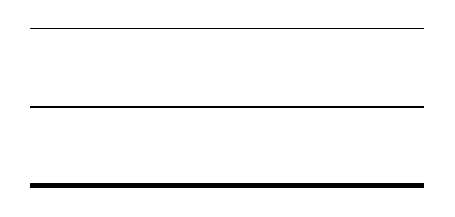
\begin{tikzpicture}
\draw (0,0)--(5,0);
\draw[line width = 1pt] (0,-1)--(5,-1);
\draw[line width = 2pt] (0,-2)--(5,-2);
\end{tikzpicture}
\end{tcblisting}

TikZ 的預設值是 0.4pt

\subsection{箭頭}

可以利用 > 與 < 來指定箭頭的形式

\begin{tcblisting}{listing side text}
\begin{tikzpicture}
\draw[-] (0,0)--(5,0);
\draw[<-] (0,-1)--(5,-1);
\draw[->] (0,-2)--(5,-2);
\draw[<->] (0,-3)--(5,-3);
\draw[|->] (0,-4)--(5,-4);
\draw[|<->|] (0,-5)--(5,-5);
\draw[|-|] (0,-6)--(5,-6);
\draw[->|] (0,-7)--(5,-7);
\draw[>->>] (0,-7)--(5,-7);
\end{tikzpicture}
\end{tcblisting}

上圖是一些示範

\subsection{預定義好的樣式}

TikZ 也有預先定義好一些樣式,讓我們可以使用

\begin{tcblisting}{listing side text}
\begin{tikzpicture}
\draw[dotted] (0,0)--(5,0);
\draw[densely dotted] (0,-1)--(5,-1);
\draw[loosely dotted] (0,-2)--(5,-2);
\draw[dashed] (0,-3)--(5,-3);
\draw[densely dashed] (0,-4)--(5,-4);
\draw[loosely dashed] (0,-5)--(5,-5);
\end{tikzpicture}
\end{tcblisting}

\subsection{平移、縮放與旋轉}

可以利用 shift 來達成平移的效果

\begin{tcblisting}{listing side text}
\begin{tikzpicture}
\draw (0,0) rectangle (1,1);
\draw[shift={(2,0)}] (0,0) rectangle (1,1);
\draw[shift={(2,2)}] (0,0) rectangle (1,1);
\draw[shift={(0,2)}] (0,0) rectangle (1,1);
\draw[shift={(-2,2)}] (0,0) rectangle (1,1);
\draw[shift={(-2,0)}] (0,0) rectangle (1,1);
\draw[shift={(-2,-2)}] (0,0) rectangle (1,1);
\draw[shift={(0,-2)}] (0,0) rectangle (1,1);
\draw[shift={(2,-2)}] (0,0) rectangle (1,1);
\end{tikzpicture}
\end{tcblisting}

\begin{itemize}
\item 第二個正方形的左下頂點由 (0,0) 移到了 (2,0)
\item 第三個正方形的左下頂點由 (0,0) 移到了 (2,2)
\item 第四個正方形的左下頂點由 (0,0) 移到了 (0,2)
\item 第五個正方形的左下頂點由 (0,0) 移到了 (-2,2)
\item 第六個正方形的左下頂點由 (0,0) 移到了 (-2,0)
\item 第七個正方形的左下頂點由 (0,0) 移到了 (-2,-2)
\item 第八個正方形的左下頂點由 (0,0) 移到了 (0,-2)
\item 第九個正方形的左下頂點由 (0,0) 移到了 (2,-2)
\end{itemize}

也可以在 shift 前加上 x 或 y 來決定平移的方向,但在這種情況下就不能使用內建的長度單位,需要自行指定

\begin{tcblisting}{}
\begin{tikzpicture}
\draw (0,0) rectangle (1,1);
\draw[xshift=100pt] (0,0) rectangle (1,1);
\draw[xshift=-100pt] (0,0) rectangle (1,1);
\draw[yshift=100pt] (0,0) rectangle (1,1);
\draw[yshift=-100pt] (0,0) rectangle (1,1);
\end{tikzpicture}
\end{tcblisting}

旋轉則需要利用 rotate

\begin{tcblisting}{}
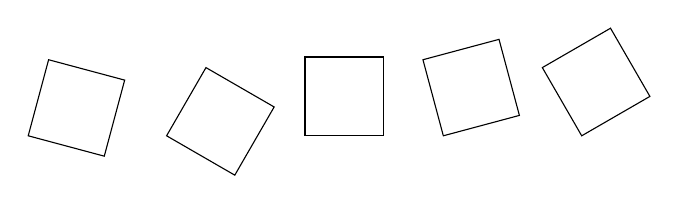
\begin{tikzpicture}
\draw (0,0) rectangle (1,1);
\draw[xshift=100pt, rotate=30] (0,0) rectangle (1,1);
\draw[xshift=50pt, rotate=15] (0,0) rectangle (1,1);
\draw[xshift=-100pt, rotate=-15] (0,0) rectangle (1,1);
\draw[xshift=-50pt, rotate=-30] (0,0) rectangle (1,1);
\end{tikzpicture}
\end{tcblisting}

\section{進階使用}

\subsection{節點}

在 \TikZ\ 中可以利用 \verb`\node(name) at(x,y) {text};` 放置節點

\begin{tcblisting}{listing side text}
\begin{tikzpicture}
\draw[help lines] (-2,-2) grid (2,2);
\node(1) at(0,0) {原點};
\end{tikzpicture}
\end{tcblisting}

想要連接兩個節點時,可以將座標改為兩個節點的名字

\begin{tcblisting}{listing side text}
\begin{tikzpicture}
\node(A) at(0,0) {A};
\node(B) at(2,0) {B};
\node(C) at(0,2) {C};
\draw (A)--(B)--(C);
\end{tikzpicture}
\end{tcblisting}

\verb`\node `如同 \verb`\draw `也可以使用選項來調整樣式

\begin{tcblisting}{listing side text}
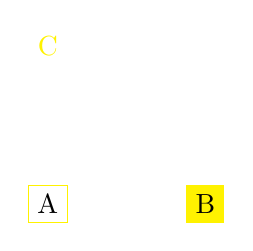
\begin{tikzpicture}
\node[draw=yellow](A) at(0,0) {A};
\node[fill=yellow](B) at(2,0) {B};
\node[text=yellow](C) at(0,2) {C};
\end{tikzpicture}
\end{tcblisting}

當然也有一些是只能用在 \verb`\node `上的選項

\begin{tcblisting}{listing side text}
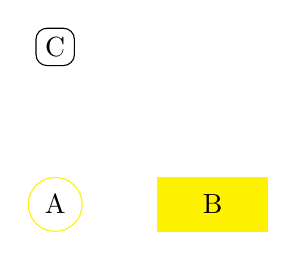
\begin{tikzpicture}
\node[draw=yellow,circle](A) at(0,0) {A};
\node[fill=yellow, minimum width=40pt, minimum height=20pt](B) at(2,0) {B};
\node[draw=black, rounded corners](C) at(0,2) {C};
\end{tikzpicture}
\end{tcblisting}

\begin{itemize}
\item 第一個節點用 circle 將外匡變成圓形的
\item 第二個節點用 minimum width/height 定義節點的最小長寬
\item 第三個節點用 rounded corners 把節點的邊角轉成圓角
\end{itemize}

但有時候我們並不想要直接把節點放到指定的座標,而是想放到該座標的上下左右,這個時候也可以利用 \TikZ\ 內建的選項來達成

\begin{tcblisting}{listing side text}

\begin{tikzpicture}
\node[left] at(0,0) {left};
\node[right] at(0,0) {right};
\node[above] at(0,0) {above};
\node[below] at(0,0) {below};
\draw[fill=black] (0,0) circle (.1);
\end{tikzpicture}
\end{tcblisting}

\begin{itemize}
\item 第一個節點在 (0,0) 的左邊
\item 第二個節點在 (0,0) 的右邊
\item 第三個節點在 (0,0) 的上方
\item 第四個節點在 (0,0) 的下方
\end{itemize}

\subsection{自定義樣式}

如果你圖片裡的節點畫線條都有相似的共同點,你可以在\verb`\begin{tikzpicture}` 後加一個方括號,並將共通的選項放在方括號中

\begin{tcblisting}{listing side text}
\begin{tikzpicture}[text = red]
\node[left, fill = yellow] at(0,0) {left};
\node[right, draw = black, line width =1pt] at(0,0) {right};
\node[above, text = blue] at(0,0) {above};
\node[below, draw = blue, circle] at(0,0) {below};
\end{tikzpicture}
\end{tcblisting}

如果你有一個很複雜的樣式,但又不是共通的,你可以利用 \verb`\tikzset{}` 來將複雜的樣式定義成一個選項

\begin{tcblisting}{listing only}
\tikzset{mynode/.style = {
draw = gray!70!black,
line width = 0.8pt,
fill = blue!30,
rounded corners,
inner sep = 6pt, %文字與邊匡的距離
minimum width = 40pt,
minimum height = 20pt}
}
\end{tcblisting}

使用時只要用 \verb`\node[mynode]` 即可

\tikzset{mynode/.style = {
draw = gray!70!black,
line width = 0.8pt,
fill = blue!30,
rounded corners,
inner sep = 6pt, %文字與邊匡的距離
minimum width = 40pt,
minimum height = 20pt}
}
\begin{tcblisting}{}
\begin{tikzpicture}[->, line width = 2pt]
\node[mynode] (1) at (0,0) {First Thing};
\node[mynode] (2) at (3,0) {Second Thing};
\node[mynode] (3) at (6,0) {Third Thing};
\draw (1)--(2);
\draw (2)--(3);
\end{tikzpicture}
\end{tcblisting}

這樣就方便許多了

\subsection{函數圖}

畫函數一樣是使用 \verb`\draw ` 這個命令

\begin{tcblisting}{}
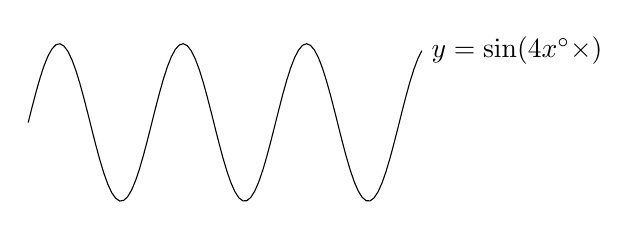
\begin{tikzpicture}
\draw[domain = 0:5, samples = 100] plot (\x,{sin(deg(\x*4))}) node[right] {$y=\sin(4x^\circ \times)$};
\end{tikzpicture}
\end{tcblisting}

domain 是我們要畫的區間,起點與終點要用冒號隔開,samples 決定圖形的精細程度,要特別注意的是需要運算的部分需要放在 \verb`{}`之間

\begin{figure}[htp]
\includegraphics[width=0.75\textwidth]{TikZ.png}
\end{figure}

上圖是可以使用的運算子,不過更複雜的函數圖形 \TikZ 就很難畫出來了,所以下一篇會介紹 pgfplots 這個 package
\newpage%%tikz
\chapter{pgfplots}

pgfplots 是一個可以畫出複雜的三維圖表的強大 Package,需要注意的是這個 Package 是基於前面介紹過的 \TikZ\ ,所以在使用之前請記得要先使用 \TikZ 。

\section{簡介}

在使用 pgfplots 之前我們需要先使用 tikzpicture 環境,之後再使用 pgfplots  提供的 axis 環境。

\begin{tcblisting}{}
\begin{tikzpicture}
\begin{axis}
......
\end{axis}
\end{tikzpicture}
\end{tcblisting}

我們要將 pgfplots 提供的命令放在 axis 環境中,第一個要介紹的是  \verb`\addplot` 這個命令,大部分可選參數是與 \TikZ 的可選參數相同,方程式則是與大部分程式語言的表達方式一樣。

\begin{tcblisting}{}
%\addplot[可選參數]{方程式}
\begin{tikzpicture}
\begin{axis}
\addplot[domain=-5:5, color=blue] {x^2};
\end{axis}
\end{tikzpicture}
\end{tcblisting}

使用完之後也請不要忘記在最後面加上 ;。

\section{二維圖形}

\subsection{函數圖}

第一個介紹的還是函數圖,簡單的範例上面展示過了,所以這裡會比較注重在介紹不同的可選參數。

\begin{tcblisting}{}
\begin{tikzpicture}
\begin{axis}
\addplot[domain=-5:5, color=blue] {x^2};
\end{axis}
\end{tikzpicture}
\end{tcblisting}

這是上面所展示的陽春例子,我們可以再多加一個方程式讓他看起來好一點。

\begin{tcblisting}{}
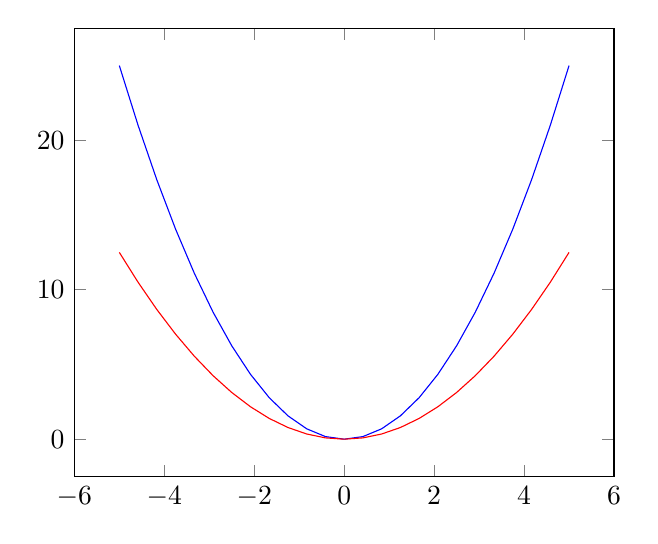
\begin{tikzpicture}
\begin{axis}
\addplot[domain=-5:5, color=blue] {x^2};
\addplot[domain=-5:5, color=red] {x^2/2};
\end{axis}
\end{tikzpicture}
\end{tcblisting}

可是這樣沒有標示難免會讓人搞混,所以我們可以利用 \verb`\addlegendentry ` 加入註解。

\begin{tcblisting}{}
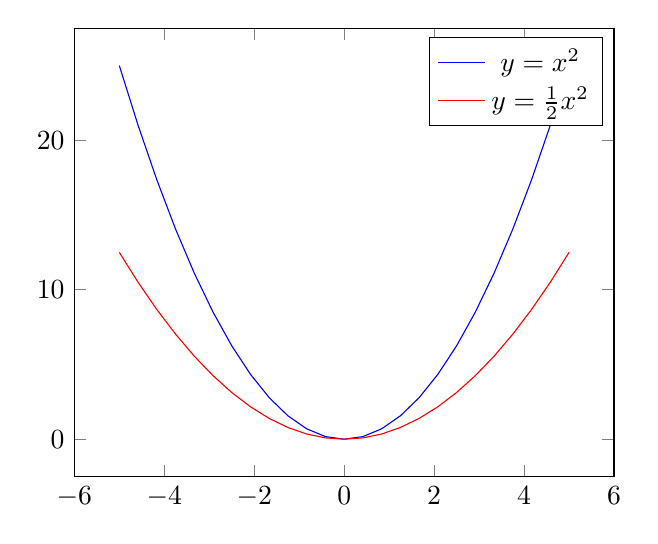
\begin{tikzpicture}
\begin{axis}
\addplot[domain=-5:5, color=blue] {x^2};
\addlegendentry{\(y=x^2\)}
\addplot[domain=-5:5, color=red] {x^2/2};
\addlegendentry{\(y=\frac{1}{2}x^2\)}
\end{axis}
\end{tikzpicture}
\end{tcblisting}

這樣就不會搞混了,如果今天想要用對數來當 x, y 軸的單位,pgfplots 也有提供 \verb`\begin{semilogxaxis}` 與 \verb`\begin{semilogyaxis}` 來解決這個問題。

\begin{tcblisting}{}
\begin{tikzpicture}
\begin{semilogyaxis}
\addplot[domain=-10:10, color=blue, samples=1000] {log10(x)};
\end{semilogyaxis}
\end{tikzpicture}
\end{tcblisting}

有時候座標軸會不符合我們想要的樣式,這時可以利用 axis lines 來調整。

\begin{tcblisting}{}
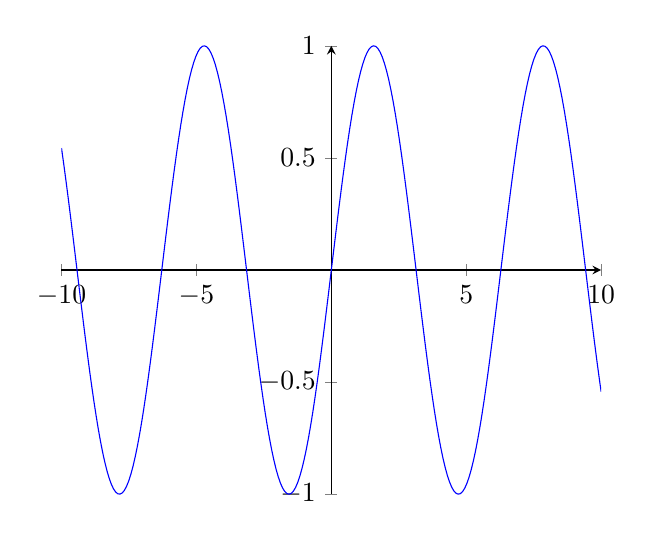
\begin{tikzpicture}
\begin{axis}[axis lines = middle]
\addplot[domain=-10:10, color=blue, samples=250] {sin(deg(x))};
\end{axis}
\end{tikzpicture}
\end{tcblisting}

\subsection{折線圖}

除了函數圖外,pgfplots 也可以繪製折線圖。

\begin{tcblisting}{}
\begin{tikzpicture}
\begin{axis}
\addplot coordinates{(0,0)(1,4)(2,3)(3,5)(4,2)(5,1)(6,0)(7,8)};
\end{axis}
\end{tikzpicture}
\end{tcblisting}

在 coordinates 後面的將放入所有折線圖的點,就可以畫出折線圖了,但有時座標軸上的標記與想像中的並不一樣,這時就需要用 xtick 與 ytick 調整。

\begin{tcblisting}{}
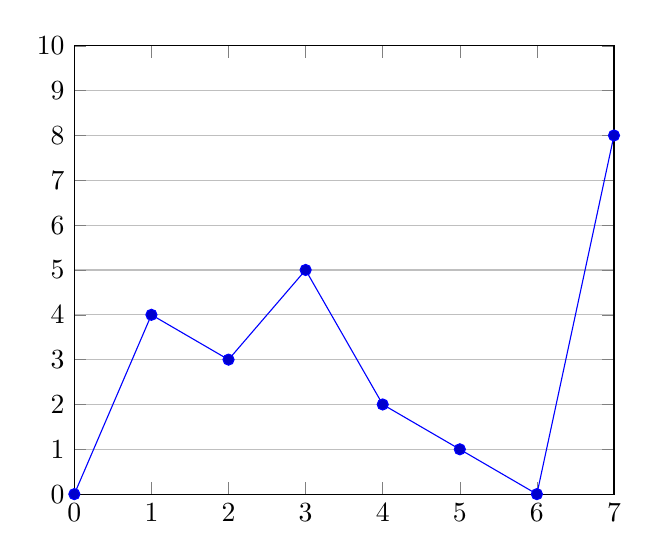
\begin{tikzpicture}
\begin{axis}[
xmin=0, xmax=7,
ymin=0, ymax=10,
xtick={0,1,2,3,4,5,6,7},
ytick={0,1,2,3,4,5,6,7,8,9,10},
ymajorgrids=true,
]
\addplot coordinates{(0,0)(1,4)(2,3)(3,5)(4,2)(5,1)(6,0)(7,8)};
\end{axis}
\end{tikzpicture}
\end{tcblisting}

\begin{itemize}
\item xmin, ymin, xmax, ymax 這些是指定 x 軸與 y 軸的最大、最小值
\item xtick, ytick 是指定 x 軸與 y 軸上的標記的位置
\item ymajorgrids 是繪製出與 y 軸相交的格線,可以用 xmajorgrids 來繪製出與 x 軸相交的格線,或用 grids=major 同時繪製兩者。
\end{itemize}

\subsection{長條圖}

長條圖與折線圖有者異曲同工之妙

\begin{tcblisting}{}
\begin{tikzpicture}
\begin{axis}[ybar, ybar interval=0.75, enlargelimits=0.1]
\addplot coordinates{(2040,9.50)(2030,10.60) (2020,12.58)};
\addplot coordinates{(2020,17.50) (2030,24.10) (2040,30.60)};
\legend{0~14歲人口所占比率(\%),65歲以上人口所占比率(\%)}
\end{axis}
\end{tikzpicture}
\end{tcblisting}

\begin{itemize}
\item ybar 指的是長條與 y 軸平行,另外還有 xbar 這個選項可以用。
\item ybar interval 是指定長條之間的空隙,1 代表沒有空隙。
\item enlarge limits 是調整整個座標軸與圖表的元素間的距離,另外也可以用enlarge x limits, enlarge y limits 等等來單獨調整特定的座標軸。
\end{itemize}

\subsection{散佈圖}

散佈圖也很簡單。

\begin{tcblisting}{}
\begin{tikzpicture}
\begin{axis}
\addplot[scatter, mark=*, only marks]
coordinates{(143,62) (50,594) (165,53) (139,348) (145,194) (75,533) (51,258) (154,492)};
\end{axis}
\end{tikzpicture}
\end{tcblisting}

\begin{itemize}
\item scatter 是讓顏色依據 y 軸的數值而變化
\item only marks 是不讓點之間用線連起來
\item mark 是指定點的標記的樣式
\end{itemize}

\subsection{從其他檔案輸入數據}

上面的方法這只適用於數據只有寥寥幾筆時,不然如果有一千多筆,一個一個 key 未免太過勞神費力,不過 pgfplots 都幫你想好了,他可以讓你從 .dat 或 .csv 檔中輸入數據。

\begin{tcblisting}{}
\begin{tikzpicture}
\begin{axis}[x tick label style={/pgf/number format/1000 sep=},width=10cm, grid=major]
\addplot table [x=year, y=youth, col sep=comma, mark=none] {data.csv};
\addlegendentry{0~14歲人口所占比率(%)}
\addplot table [x=year, y=old, col sep=comma, mark=none] {data.csv};
\addlegendentry{65歲以上人口所占比率(%)}
\end{axis}
\end{tikzpicture}
\end{tcblisting}

\begin{itemize}
\item x tick label style 是調整 x 軸上標示的樣式。
\item table 是表示資料來源是類似表格的形式。
\item x=, y= 是指定 x, y 的數據要從哪一欄輸入。
\item col sep 是告訴 pgfplots 欄與欄的分界是用什麼符號。
\end{itemize}

\section{三維圖形}

終於進入三維圖形了,三維圖形的繪製方式與二維圖形相似,只是命令要改用 \verb`\addplot3` 這個命令外,其他的選項幾乎都通用。

\begin{tcblisting}{}
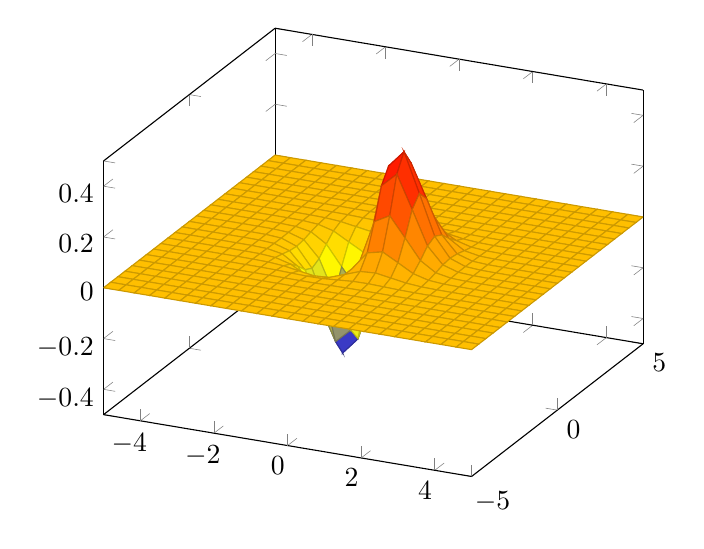
\begin{tikzpicture}
\begin{axis}
\addplot3[surf] {exp(-x^2-y^2)*x};
\end{axis}
\end{tikzpicture}
\end{tcblisting}

surf 是 surface 的縮寫與 scatter 有異曲同工之妙,同樣會因為某一軸的數值高低而產生顏色變化。\newpage%%pgfplots
\chapter{用 Beamer 做簡報}

如果想要用 \LaTeX\ 製作簡報,可以利用 beamer 這個文件類型來製作,不只可以做差一張張的靜態投影片,也可以創造出一點點的動畫效果

\subsection{基礎使用}

一個簡單的 beamaer 範例

\begin{tcblisting}{listing only}
\documentclass{beamer} %使用 beamer 為文件類型
\usepackage{xeCJK}
\setCJKmainfont{TW-Kai}
\author{Si manglam}
\title{如何使用 Beamer}
\subtitle{Beamer 大作戰}
\institute{IT 邦幫忙}
\date{2022/09/10}
\begin{document}
\begin{frame}
\titlepage
\end{frame}
\begin{frame}
\frametitle{標題}
\end{frame}
\end{document}
\end{tcblisting}

\begin{itemize}
\item frame 環境創造了新的投影片,所有要在投影片上的內容都要在這個環境內
\item \verb`\titlepage` 自動輸出標題頁
\item \verb`\frametitle`	為當前投影片加入標題
\end{itemize}

如果作者並不只有一個人且來自不同機構,我們需要用微調來讓投影片更美觀

\begin{tcblisting}{listing only}
\title[重大發現]{一個足以改變人類未來的重大發現}
\author[Luke \& manglam]{Si manglam\inst{1} \and Luke\inst{2}}
\institute[實驗室、知名大學]{\inst{1}不具名的實驗室 \and \inst{2}某間知名大學}
\date[22xx 知名會議]{22xx/xx/xx某知名會議}
\end{tcblisting}

上面的例子中,兩個作者與兩個機構中間都用\verb`\and ` 隔開,方括號內的則是在其他地方顯示的,現在可能還看不出差別,但看到下面用 \verb`\usetheme{}` 來使用 beamer 內建主題的範例就可以看出明顯的差異了

\begin{tcblisting}{listing only}
\usetheme{Madrid}
\begin{document}
\begin{frame}
\titlepage
\end{frame}
\begin{frame}
\frametitle{標題}
\end{frame}
\end{document}
\end{tcblisting}

可以看到這樣美觀了許多,同時方括號的內容顯示在下面那排,更多的主題可以在<連結>中找到

\section{小技巧}

beamer 與一般的文件一樣可以用 \verb`\tableofcontents `來建立目錄

<圖片>

也可以利用 \verb`\tableofcontents[currentsection]`來明確的標示現在的章節

<圖片>

beamer 也有針對投影片用途新定義一些環境

\begin{tcblisting}{listing only}
\begin{block}{這是一個 block}
文字
\end{block}

\begin{alertblock}{特別注意}
文字文字文字文字文字
\end{alertblock}

\begin{examples}
文字文字文字文字文字
\end{examples}
\end{tcblisting}

雖然 beamer 的主題有限,但只要換個色系就不會有人發現了

\begin{tcblisting}{listing only}
\usetheme{Madrid}
\usecolortheme{seahorse}
\end{tcblisting}

\section{overlay}

利用 \verb`\only<頁數>{}` 與 \verb`\discover<頁數>{}` 可以控制元素出現的時機,兩者差別在一個是只在特定頁數出現,一個是隱形且只會在特定頁數出現。

\begin{tcblisting}{listing only}
\begin{center}
A\only<1>{第一頁出現}\\
A\discover<1-2>{第一、二頁}\\
A\only<2-3>{第二、三頁}\\
A\discover<3>{第三頁}\\
\end{center}
\end{tcblisting}

如果是想要讓條列的內容一條條出現可以直接在用 \verb`\begin{itemize}[<+->]`

\begin{tcblisting}{listing only}
\begin{itemize}[<+->]
\item 一
\item 二
\item 三
\end{itemize} 
\end{tcblisting}

但如果要特別指定頁數,就要在 \verb`\item `後加 <頁數>

\begin{tcblisting}{listing only}
\begin{itemize}[<+->]
\item<1-> 一
\item<2> 二
\item<3-4> 三
\item<4> 四
\item<5> 五
\end{itemize} 
\end{tcblisting}

可以看到有三出現在兩頁,這些就是 beamer 如何控制 Overlay。\newpage%%Beamer
\chapter{biblatex}

biblatex 是一個管理參考文獻的 package,他可以幫助我們方便快速的管理參考文獻。

\section{前置作業}

首先我們需要準備 .bib 檔, .bib 檔的基礎形式如下

\begin{tcblisting}{listing only}
@Article{key,
author = {作者},
title = {標題},
journal = {期刊},
year = {年份},
}
\end{tcblisting}


\verb`@Article` 是宣告參考文獻是期刊中的文章,key 是在文章中引用連結使用的,但通常我們不用親自撰寫 .bib 檔,因為像 Google Scholar 之類的文獻資料庫都會提供 bibtex 的格式。

圖片

上圖是如何在 Google Scholar 取得 .bib 檔的方式。

\section{基礎使用}

在準備好 .bib 檔後就可以開始使用 biblatex 了,首先我們需要告訴 biblatex 我們的 .bib 檔叫什麼名字。

\begin{tcblisting}{listing only}
%\usepackage{biblatex}
\addbibresource{name.bib}
\end{tcblisting}

利用 \verb`\addbibresource{•}` 告訴 biblatex .bib 檔的名稱後,我們就可以利用 \verb`\cite{key}` 在文章中引用參考文獻了。

\begin{tcblisting}{listing only}
Free software 跟價錢並沒有關係,這裡的 Free 指的是自由。\cite{stallman2002free}
\end{tcblisting}

如果不是使用 overleaf 的人需要注意,我們需要額外跑一次 bibber 和兩次 \LaTeX ,順序如下:

\begin{enumerate}
\item \LaTeX
\item biber
\item \LaTeX 
\item \LaTeX
\end{enumerate}

這樣就可以引用參考文獻了,但我們還需要用 \verb`\printbibliography` 將有用到的參考資料都列出來。

\begin{tcblisting}{listing only}
\printbibliography
\end{tcblisting}

這樣所有被引用過的資料就都被列出來了,如果有參考文獻沒有被直接引用,又想要讓他出現在此,需要用 \verb`\nocite{key}` 將他列出來。

\begin{tcblisting}{listing only}
Free software 跟價錢並沒有關係,這裡的 Free 指的是自由。\cite{stallman2002free}
\nocite{key}
\printbibliography
\end{tcblisting}

如果想將檔案中所有的參考文獻都列出,只需將 key 換成 * 就好了,如果引用了許多文章,但最後在列出時想要分類這一大群的參考文獻時,有兩種方法,第一種是利用 \verb`type=` 來依照參考文獻的類型分類。

\begin{tcblisting}{listing only}
\printbibliography[type=article, title=article]
\printbibliography[type=book, title=book]
\end{tcblisting}

第二個方法是在撰寫 bib 檔時加入 \verb`keywords` ,以便分類。

\begin{tcblisting}{listing only}
\printbibliography[keyword=LaTeX, title=article]
\printbibliography[keyword=Overleaf, title=book]
\end{tcblisting}

\begin{tcblisting}{listing only}
@book{stallman2002free,
  title={Free software, free society: Selected essays of Richard M. Stallman},
  author={Stallman, Richard},
  year={2002},
  publisher={Lulu. com},
  keywords={}
}
\end{tcblisting}

如果想要更進一步的了解 biblatex 到底可以做什麼,可以參考以下幾篇文章。
\newpage%%biblatex
\chapter{animate}

有時候人總是要會一兩招華而不實的招數,好在需要的時候秀一手,我們可以藉由在 pdf 中加入 gif 動畫以達到上述的效果。

\section{基礎使用}

在使用之前需要先在導言區載入 graphicx package,在載入之後我們就可以利用  \verb`\animategraphics{}{}{}{}` 來插入動畫,但在插入動畫之前,我們需要先了解 animate 是如何插入動畫的,實際上 animate 並不能將 gif 直接塞入 pdf 中,他是利用 javascript 讓 pdf 中的圖片可以動起來,所以在拿到 gif 後我們還需要將 gif 轉成其他格式。

\subsection{格式轉換}

我們需要使用各種手段將 gif 轉換成 png 或 jpeg 等,可以使用 ImageMagick 這個工具來轉換,在安裝好之後可以在終端機用 convert 命令來轉換格式,

\begin{tcblisting}{listing only}
convert input.gif -coalesce output.png
\end{tcblisting}

可以利用這行命令將 gif 改成一系列的圖片。

\subsection{正式使用}

\begin{tcblisting}{listing only}
\animategraphics[autoplay]{.5}{A-}{1}{5}
\end{tcblisting}

\begin{itemize}
\item 前面中括號內放可選參數
\item 第一個花括號是指定動畫的幀數
\item 第二個花括號是檔案的前綴名
\item 第三個花括號是檔案的開頭、第四個則是結束,這條指令會將 A-1, A-2, A-3, A-4, A-5 作為動畫的
\end{itemize}

這裡有一系列的可選參數

\begin{itemize}
\item autoplay: 當滑到動畫所在的頁面時自動播放
\item loop: 不斷重複播放動畫
\item palindrome: 在動畫播放完後倒帶動畫,並重新循環
\item step: 將動畫的放映模式改成點一下播一張
\item controls: 決定動畫下的播放按鈕
\item label: 給定一個 javascript 的標籤
\end{itemize}

\subsection{自行繪製}

隨意使用網路上的 gif 圖可能會有版權相關的問題,但好在我們可以利用 animateinline 環境來自行繪製。

\begin{tcblisting}{listing only}
\begin{animateinline}[begin={\begin{tikzpicture}\draw (-1,-1) rectangle (3.5,1);}end={\end{tikzpicture}}]{0.5}
\draw (0,0)--(0.5,0);
\newframe
\draw (0,0)--(1,0);
\newframe
\draw (0,0)--(1.5,0);
\newframe
\draw (0,0)--(2,0);
\newframe
\draw (0,0)--(2.5,0);
\newframe
\draw (0,0)--(3,0);
\newframe
\draw (0,0)--(3.5,0);
\end{animateinline}
\end{tcblisting}

\begin{itemize}
\item begin 跟 emd 是指在每一幀之前自動插入的命令
\item 整個動畫的大小是依據第一幀的大小來進行縮放的,所以我在每一幀都加入了看不見的正方形以維持動畫大小的一致性
\end{itemize}

當然這些只是簡單的範例,只要你想得到,沒有什麼是你做不出來的。\newpage%%animate
\chapter{lualatex}

Lua\LaTeX 是將 Lua 與 \TeX\ 結合在一起,讓改動 \TeX\ 的排版規則時可以不用 \TeX ing,更詳細的使用需要對 Lua\TeX 與 \LaTeX\ 有深刻的認識,目前我的能力還不到這麼深厚,所以我只介紹一些基礎的用法。

\section{基礎用法}

想要在 Lua\LaTeX 裡使用 Lua 需要透過 \verb`\directlua{}` 的協助,這個命令會將花括號中命令轉給 Lua 解釋器,要想讓 Lua 產出的結果可以轉回給 \LaTeX 需要用 \verb``tex.sprint`。

\begin{tcblisting}{listing only}
tex.sprint("$\cos(0)$等於".. math.cos(math.rad(0)))
\end{tcblisting}

執行之後可以看到 $\cos$ 被輸出出來了,這就是基礎的 Lua\LaTeX 的用法更進階的也可以將 for 迴圈帶入使用

\begin{tcblisting}{listing only}
\directlua{
tex.sprint("\\begin{tabular}{|c|c|c|}")
tex.sprint("\\hline")
tex.sprint("x & sin(x) & cos(x) \\\\ ")
tex.sprint("\\hline")
for x = 0,180,10 do
	tex.sprint(x .." & ".. math.sin(math.rad(x)) .." & ".. math.cos(math.rad(x)) .." \\\\ ")
	tex.sprint("\\hline")
end
tex.sprint("\\end{tabular}")
}
\end{tcblisting}

執行後可以看到有表格被產出了,如果有什麼重複性高的指令,也可以用這種方式來節省時間,這是基礎的 Lua\LaTeX 的使用方法。

\section{進階使用}

進階使用我也不會所以在這裡放一個我看到的例子:

\begin{tcblisting}{listing only}
function fadelines(head)
        GLYPH = node.id("glyph")
        WHAT = node.id("whatsit")
        COL = node.subtype("pdf_colorstack")
        colorize = node.new(WHAT,COL)
        cvalue = 0
        for line in node.traverse_id(GLYPH,head) do
            colorize.data = cvalue.." "..1 - cvalue.." .5".." rg"
            node.insert_before(head, line, node.copy(colorize))
            cvalue = math.min(cvalue + .0008, 1)
        end
        return head
    end

    luatexbase.add_to_callback("pre_linebreak_filter", fadelines, "fadelines")
\end{tcblisting}

這樣產生的結果如下圖:

\begin{figure}[htp]
\centering
\includegraphics[width=0.75\textwidth]{sampla.pdf}
\end{figure}

要達成這種效果,需要對 Lua\LaTeX 以及 \LaTeX 有著即為深厚的認識。\newpage%%lualatex
\chapter{LuaLaTeX 做動畫}

繼上一篇介紹了 Lua\LaTeX 後,相信大家都瞭解了 Lua\LaTeX 的基本使用方式,今天要教大家的則是如何用 Lua\LaTeX 加上 animate 製作動畫,特別提醒:這不是正常的 Lua\LaTeX 的使用方法。

\section{基礎創作}

基本上最常使用到的環境大概是物件的移動,我們不太可能一幀幀的繪製出物件的移動軌跡,因為那樣程式碼會顯得過於冗長,所以我們可以利用 for 迴圈去縮減程式碼。

\begin{tcblisting}{listing only}
\begin{luacode}
tex.sprint("\\begin{animateinline}[autoplay,loop]{10}")
for x = -4,4,0.1 do
	tex.sprint("\\begin{tikzpicture}")
	tex.sprint("\\draw[color=white] (-5,-5) rectangle (5,5);")
	tex.sprint("\\draw[fill=black] (".. x ..",0) circle (0.5);")
	tex.sprint("\\end{tikzpicture}")
	tex.sprint("\\newframe")
end
tex.sprint("\\end{animateinline}")
\end{luacode}
\end{tcblisting}

編譯出來的動畫是一個小球漸漸的從左移到右,比起一幀幀繪製,這樣簡單多了。

\section{進階創作}

更進階的創作用法可以再加上 if 迴圈,例如以下的動畫:

\begin{tcblisting}{listing only}
\begin{luacode}
tex.sprint("\\begin{animateinline}[autoplay,loop]{10}")
for x = 0,360,5 do
	tex.sprint("\\begin{tikzpicture}")
	tex.sprint("\\draw[color=white] (-2,-2) rectangle (2,2);")
	if (math.sin(math.rad(x)) > 0) then
		tex.sprint("\\draw[fill=red] (0,".. math.sin(math.rad(x)) ..") circle (0.5);")
	else
		tex.sprint("\\draw[fill=blue] (0,".. math.sin(math.rad(x)) ..") circle (0.5);")
	tex.sprint("\\end{tikzpicture}")
	tex.sprint("\\newframe")
end
tex.sprint("\\end{animateinline}")
\end{luacode}
\end{tcblisting}

編譯出的結果是一個會隨著高度變換顏色的小球,更多的使用方法就要靠你們自己去發想了,只要是有規律地動會,都可以用這種方式繪製出來的。\newpage%%lualatex 做動畫
\chapter{自定義命令與環境}

在看完了這麼多的 package 後,你會發現有時候為了追求美觀,可能會需要利用到大量的命令去調整輸出,如果只使用一次那還好說,但如果需要在文件中不斷地使用到這個功能,不斷重複的程式碼一來會增加 Debug 的困難度、二來還會降低效率,為了解決這種問題 \LaTeX 提供了以下四個命令來協助使用者自定義命令與環境。

\begin{itemize}
\item \verb|\newcommand{cmd}[必選參數的數量]{definition}|
\item \verb|\renewcommand{cmd}[必選參數的數量]{definition}|
\item \verb|\newenvironment{env}[必選參數的數量]{before env}{after env}|
\item \verb|\renewenvironment{env}[必選參數的數量]{before env}{after env}|
\end{itemize}

\LaTeX 是是一個大小寫敏感的程式語言,所以 \verb|\LaTeX| 與 \verb|\latex| 是有所差別的,另外 \LaTeX 在命名上不能使用數字、符號等等,所有的命令皆只能由字母組成。另外除了定義新的命令外\LaTeX 提供了兩個以 re 開頭的命令,以讓我們改寫已被定義過的命令或環境。

\section{自定義命令}

在初步了解過如何自定義命令後就可以上手試試了,如果我們在排版中需要重複使用一個複雜的樣式,例如需要一個黃底、紅字、粗體的樣式來特別標注重點,如果正常使用應該會需要將三個命令套在一起使用,先不說方便性,使用的次數一多還會降低可讀性,所以我們可以將這一連串的命令定義成一個新的命令:

\begin{tcblisting}{}
\newcommand{\important}[1]{%定義名為 \important 的命令
\colorbox{yellow}{\textcolor{red}{\textbf{#1}}}
}
這是一個非常\important{重要的公告}
\end{tcblisting}

可以看到我將 \verb|\important| 定義為一串命令,如此一來即可利用\verb|\important| 來代替一長串的命令,而在定義的過程中 \# 1代表的是必選參數一,若這個可選命令有多個必選參數,也必須以此類推,將 \# 1 一路加到 \# 9 為止,需要注意 \LaTeX 的必選參數是不可以超過 9 個的。

\section{自定義環境}

定義環境與定義命令相似,不同的點在於環境需要定義環境開始與結束時的命令,例如想要一個特殊的環境來區分引用的文字,可以從想要的呈現結果開始著手,我想要環境的上下留一點白、環境內的文字要改成斜體、還要一個必選參數將來源標示出來,請看以下的範例:

\begin{tcblisting}{listing only}
\newenvironment{poetry}[1]{%
\newcommand{\poetryfer}{#1}
\vskip6pt plus 2pt minus 2pt
\let\oldparindent\parindent
\setlength{\parindent}{0pt}
\setlength{\leftskip}{12pt}\itshape}{
\\ -\poetryfer 
\vskip6pt plus 2pt minus 2pt
\setlength{\parindent}{\oldparindent}
}
\end{tcblisting}

\begin{poetry}{邱妙津《蒙馬特遺書》}
世界總是沒有錯的,\\
錯的是心靈的脆弱性,\\
我們不能免除於世界的傷害,\\
於是我們就要長期生著靈魂的病。
\end{poetry}

上面是這個範例的結果,在這個範例中,我們定義了 poetry 環境,在環境開始之前會先由 vskip 留白,接者再利用 \verb|\let| 命令將原先的縮排長度暫存起來,而後將縮排長度改成零,最後將整段的縮進設為 12pt 字體設為斜體。在環境結束的時候,先換到下一行再將來源標示出來,要注意在第二格括號內是不能使用必選參數的,但可以先在第一個括號中儲存成命令,在第二個括號中再利用命令的方式使用。

這就是在 \LaTeX 中自定義環境與命令的方式,善用這個技巧可以確保排版的一致性也可以減少所需使用的命令數。\newpage
\chapter{etoolbox}

倒數第二天了,今天要跟大家介紹 etoolbox 這個可以讓你編輯已有命令的 package。

\section{使用之前}

因為這個 package 是讓你編輯已有命令,所以在編輯之前我們必須先找出命令的原始定義,LaTeX 提供了 \verb`\show` 這個命令來協助我們,只要在 \verb`\show`後面接上想要查詢的指令,就可以在 .log 檔中看到命令的定義,除了利用 \verb`\show` 查詢之外,我們也可以直接在原始碼中尋找定義。

不過以上兩種方式都有不便之處,\verb`\show` 無法快速的顯示出命令的定義,直接在原始碼中尋找定義又會花上大把的時間。我們急需一個更方便的方式來尋找命令的定義,latexdef 是你的一個好選擇,只要在終端機上打出 latexdef 加上你要找尋的命令即可。

\begin{tcblisting}{listing only}
latexdef TeX
\end{tcblisting}

\section{實戰}

這裡以有章節標題頁無法被自定義為例,跟章節標題有關的命令只有\verb`\chapter` 所以先讓我們看看 \verb`\chapter` 的定義:

\begin{tcblisting}{listing only}
latexdef chapter
\chapter:
undefined
\end{tcblisting}

你會發現怎麼找不到他的定義,這是因為 latexdef 預設是載入 Plain \TeX\ 格式,而不是 \LaTeX\ 格式,並且預設的文件格式是 article 所以我們還需要指定文件格式:

\begin{tcblisting}{listing only}
latexdef --tex latex -c report chapter
\chapter:
\long macro:->\if@openright \cleardoublepage \else \clearpage \fi \thispagestyle {plain}\global \@topnum \z@ \@afterindentfalse \secdef \@chapter \@schapter
\end{tcblisting}

\begin{itemize}
\item \verb`--`tex 是指定載入的格式
\item -c 是指定載入的文件類別
\end{itemize}

這樣我們就得到\verb|\chapter|的定義了,在裡面找到\verb|\thispagestyle{plain}|這個罪魁禍首,利用 etoolbox 提供的\verb|\xpatchcmd|來修改:

\begin{tcblisting}{listing only}
%\xpatchcmd{命令}{修改前內容}{修改後內容}{ }{ }
\xpatchcmd{\chapter}{\thispagestyle{plain}}{ }{ }{ }
\end{tcblisting}

這樣就可以讓標題頁的樣式是自定義的樣式了。這也是簡單修改命令定義的方式。\newpage%%etoolbox
\chapter{繼續前行}

這篇就不再寫技術相關的內容了,而要來介紹哪裡可以找到更多關於 \LaTeX\ 的資料,畢竟書本的內容有限,且學習不能一直閉門造車。

\section{網頁}

以下幾個網頁是我很推薦的資料來源

\begin{itemize}
\item CTAN
\item Overleaf
\item Stack Exchange
\end{itemize}

CTAN 是 Comprehensive TeX Archive Network 的縮寫,基本上只要是 \TeX\ 有關的資料都會被收藏在此(\LaTeX\ 當然也被包含在內),如果有什麼 package 或使用手冊想要找,甚至是自己寫了一個 package 想要與全世界的 \TeX\ 使用者共享,只要到 CTAN 就對了。

Overleaf 不只提供了線上編譯 \LaTeX\ 的服務,他們也為了推廣 \LaTeX\ 寫了許多的技術文章,最棒的是他們的技術文章是為了初學者而設計的,所以不用怕看不懂,但想當然的內容是用英文寫的。

大部分人應該都聽過 Stack Exchange ,如果你有什麼問題想問,不仿先來這裡看看有沒有人問過。

如果有相關的問題,可以先去這些地方尋找答案。

\section{書籍}

書籍有以下幾本

\begin{itemize}
\item The \TeX\ book
\item The Not So Short Introduction to LATEX2ε
\item 簡單高效 \LaTeX
\item 大家來學 \LaTeX
\end{itemize}

The \TeX\ Book 是由高德納教授親自編寫的書籍,可以說是血統純正,但內容主要是介紹 \TeX\ 的的功能,比較適合想要了解 \LaTeX\ 系統底層的人,不建議初學者質監研讀此本書。

簡單高效 \LaTeX\ 與大家來學 \LaTeX\ 皆為中文書籍,是在資源缺乏的中文圈中為數不多的寶藏資料,兩篇皆以精簡的篇幅介紹了 \LaTeX\ 的基礎使用,並且也廣泛的介紹 \LaTeX\ 中常用的 package。 

\newpage%%繼續前行
\chapter{Beyond LaTeX}

終於完稿了,當初會想寫下這本書可說全部都是意外,事情得要從一個地科作業開始說起,當時在寫地科作業的我正被「如何在 page 內加入數學方程式」而困擾著,於是我打開了 page 內建的插入方程式功能,只見一行大字出現在視窗內「請使用 mathml 或 \LaTeX\ 來插入數學方程式」,這就是我遇見 \LaTeX\ 的過程。

後來我就開始學習 \LaTeX\ ,在學習的過程中我發現跟 \LaTeX\ 有關的中文資料只有兩種,不是簡體字就是有一定年份的資料,除了這之外就全部都是英文資料了,中文資料的缺乏讓我開始思考我可以做什麼來改善這個情況,於是我開始撰寫了這本書,希望可以為臺灣的 \LaTeX\ 社群增添一份可用的資料。

在撰寫途中不禁感嘆自己對 \LaTeX\ 瞭解的不足,同時也驚嘆於 \LaTeX\ 強大的排版功能,也讓我撰寫本書的決心更加強烈,雖然我只是一個高中生,這也只是一個自主學習的計畫,但我也是有力量的,只要我將我的力量貢獻出,某些需要幫助的人就一定能收到,最後希望各位都可以在撰寫 \LaTeX\ 一帆風順。

\begin{flushright}
周造麟-Si manglam\\
Email: qwer09214@gmail.com\\
2022/10/10 寫下
\end{flushright}\newpage%%Beyond LaTeX
\end{document}